\documentclass[11pt, xcolor={dvipsnames}, aspectratio=169]{beamer}

\usetheme{metropolis}
\usepackage{appendixnumberbeamer}
\usepackage{amsmath}
\usepackage{amssymb}
\usepackage{array}
\usepackage{mathtools}
\usepackage{caption}
\usepackage{fancyvrb}
\usepackage[separate-uncertainty]{siunitx}
\usepackage{overpic}
\usepackage{tikz}
\usepackage{booktabs}
\usepackage{multirow}
\usepackage[absolute, overlay]{textpos}
\usetikzlibrary{positioning}

\graphicspath{{logos/}{figures/}}

\titlegraphic{
  
\includegraphics[height=1.1cm]{atlas_logo}
  \hfill
  
\includegraphics[height=1.1cm]{uni_bonn_logo}
}

\setbeamercolor{background canvas}{bg=white}
\setbeamersize{text margin left=1.5em, text margin right=1.5em}

\setlength{\leftmargini}{4mm}
\setlength{\leftmarginii}{4mm}

% My definitions
\usepackage{defs}

\definecolor{headergray}{HTML}{23373B}
\definecolor{mygray}{HTML}{FAFAFA}
\definecolor{hadhadred}{HTML}{E41A1C}
\definecolor{lephadblue}{HTML}{377EB8}
\definecolor{bjetblue}{HTML}{377EB8}
\definecolor{taured}{HTML}{CC3738}
\definecolor{hhblue}{HTML}{3333FF}
\definecolor{lhred}{HTML}{CC3333}

\definecolor{toporange}{HTML}{C28B17}
\definecolor{zjetsgreen}{HTML}{0D8254}
\definecolor{fakeblue}{HTML}{6997D6}
\definecolor{topfakered}{HTML}{FE5F5A}

\author{Christopher Deutsch}
\institute{University of Bonn}
\date{June XX, 2023}

\title{\vspace{1.5em}Search for Higgs Boson Pair Production in the \bbtautau
  Final State with the ATLAS Experiment at the LHC}

\begin{document}

\maketitle

% Aim for 25ish slides?
\begin{frame}[noframenumbering]{Notes: Content}
  30 minutes (talk) + 15 minutes (discussion):
  \begin{itemize}

  \item Conclusion \& Outlook (1 slide)

  \item Event Displays (2 slides)

  \end{itemize}
\end{frame}

% ------------------------------------------------------------------------------

\begin{frame}{Introduction}
  Why do particle physics?

  What is particle physics?

  What is the origin of elementary particle masses?
\end{frame}

% ------------------------------------------------------------------------------

\begin{frame}{The Standard Model}

  \begin{columns}
    \column{0.7\textwidth}
    \centering

    \vspace*{1em}

    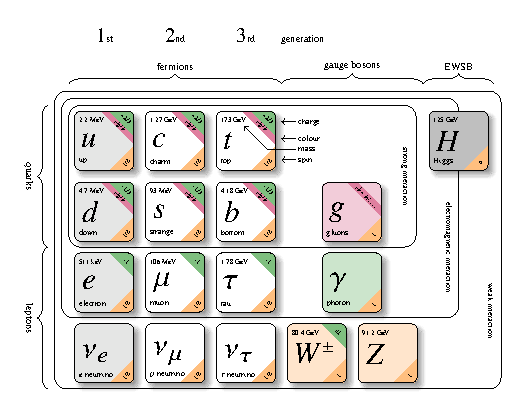
\includegraphics[width=\textwidth, trim=0.9cm 0.3cm 0.2cm 1.5cm,
    clip]{theory/sm}

    \column{0.3\textwidth}

    \begin{itemize}
      \setlength{\itemsep}{1.5em}
    \item Built on principle of local gauge invariance of the Lagrangian
    \item How to incorporate masses of elementary particles?
    \end{itemize}
  \end{columns}

  % Built on the principle of local gauge symmetries of the Lagrangian

  % Gravitation not included

  % Problem: Masses of elementary particles

\end{frame}

% ------------------------------------------------------------------------------

\begin{frame}{The Standard Model}
  \begin{center}
    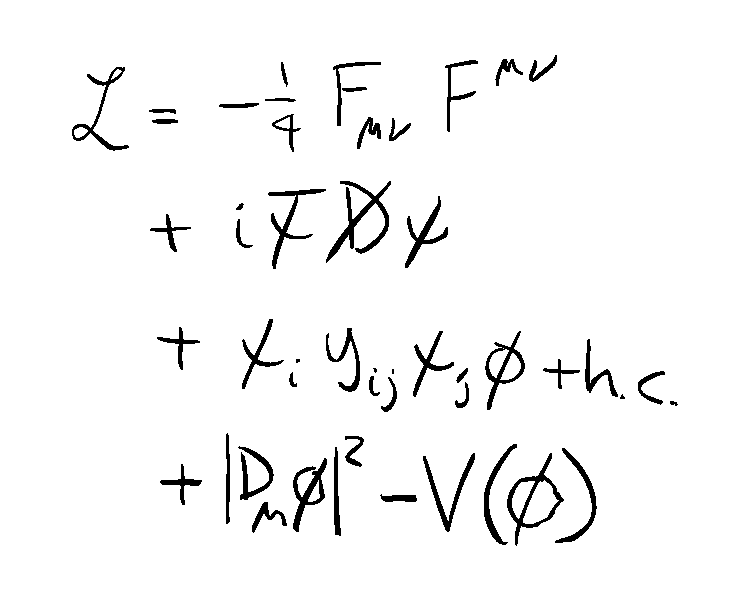
\includegraphics[width=0.6\textwidth]{lagrangian/lagrangian_vectorized}
    % Credit: CERN
  \end{center}
\end{frame}

% ------------------------------------------------------------------------------

\begin{frame}{Electroweak Symmetry Breaking}
  % Brout, Englert, Higgs -> EWSB

  \begin{columns}
    \column{0.65\textwidth}
    \centering

    % Add a (doublet) of complex scalar field with a special potential

    \begin{align*}
      V(\phi) = \mu^2 \phi^\dag \phi + \lambda (\phi^\dag \phi)^2 \\
      \mu^2 < 0
    \end{align*}

    \column{0.35\textwidth}
    \centering

    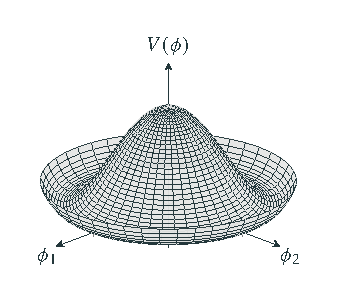
\includegraphics[width=\textwidth]{theory/potential}

    $\phi(x) = \phi_1(x) + i \, \phi_2(x)$
  \end{columns}

  \begin{align*}
    V(H) = \lambda v^2 H^2 + \lambda v H^3 + \frac{\lambda}{4} H^4
  \end{align*}
\end{frame}

% ------------------------------------------------------------------------------

\begin{frame}{Higgs Boson Discovery}

  \begin{columns}
    \column{0.5\textwidth}
    \centering

    % CERN Seminar: 4 July 2012
    \includegraphics[width=0.9\textwidth]{CERN_seminar}

    \column{0.5\textwidth}
    \centering

    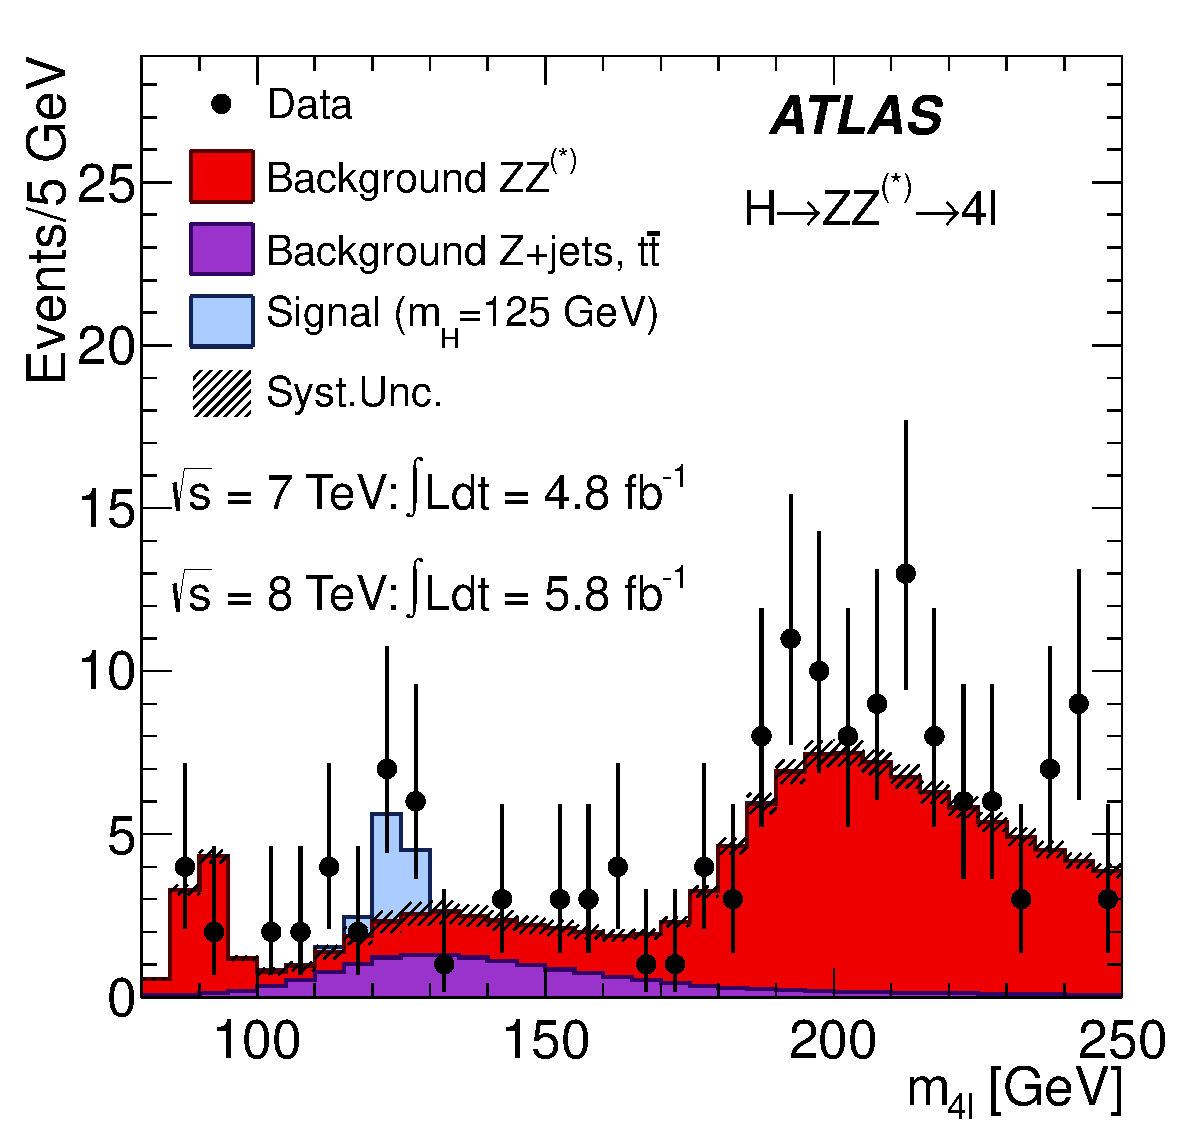
\includegraphics[width=0.55\textwidth]{higgs_discovery/fig_002}

    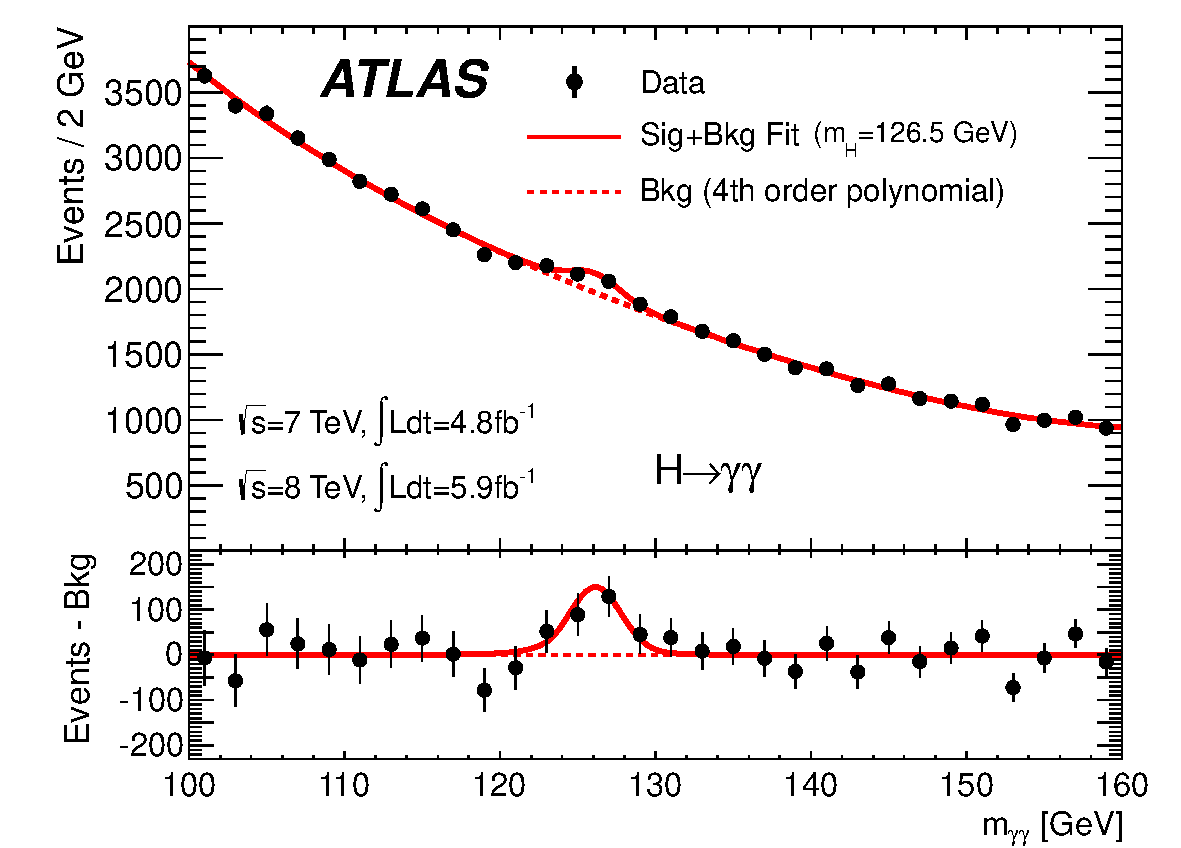
\includegraphics[width=0.7\textwidth]{higgs_discovery/figaux_004a}
  \end{columns}
\end{frame}

% ------------------------------------------------------------------------------

\begin{frame}{The Higgs Potential}

  \begin{center}
    \begin{tabular}{ccccccc}
      $V(H)$ & $=$ & ${\color{Red} \lambda v^2 H^2}$ & $+$ & ${\color{Blue} \lambda v H^3}$ & $+$ & ${\color{Green} \frac{\lambda}{4} H^4}$ \\[1.2em]
             && \raisebox{1.85em}{
\includegraphics[scale=1.0]{feynman_graphs_talk/higgs_massterm}}
             && 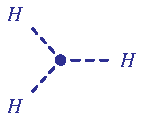
\includegraphics[scale=1.0]{feynman_graphs_talk/higgs_hhh}
             && 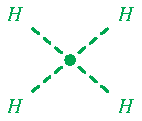
\includegraphics[scale=1.0]{feynman_graphs_talk/higgs_hhhh} \\[1.2em]
             && {\color{Red}mass term}
             && {\color{Blue}trilinear self-coupling}
             && {\color{Green}quartic self-coupling}
    \end{tabular}
  \end{center}
\end{frame}

% ------------------------------------------------------------------------------

% TODO: Make the HHH coupling red?
\begin{frame}{Higgs Boson Pair Production in the SM}
  \vspace*{0.5em}

  \fbox{%
    \noindent\begin{minipage}{\dimexpr 0.25\textwidth - 2\fboxsep}
      \centering
      \textbf{Gluon--gluon fusion}\\[0.5\baselineskip]
      $\sigma_{\HH}^{gg\text{F}} = \SI{31}{\femto\barn}$
  \end{minipage}%
  \begin{minipage}{\dimexpr 0.75\textwidth - 2\fboxsep}
    \hspace*{0.1\textwidth}
    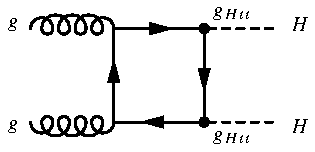
\includegraphics[scale=0.75]{feynman_graphs/di_higgs_box}%
    \hfill%
    \raisebox{0.35em}{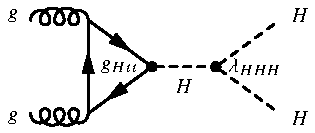
\includegraphics[scale=0.75]{feynman_graphs/di_higgs_triangle}}%
    \hspace*{0.1\textwidth}
  \end{minipage}
  }

  \vspace*{2em}

  \fbox{%
    \noindent\begin{minipage}{\dimexpr 0.25\textwidth - 2\fboxsep}
      \centering
      \textbf{Vector boson fusion}\\[0.5\baselineskip]
      $\sigma_{\HH}^{\text{VBF}} = \SI{1.7}{\femto\barn}$
    \end{minipage}%
    \begin{minipage}{\dimexpr 0.75\textwidth - 2\fboxsep}
      \hspace*{0.04\textwidth}%
      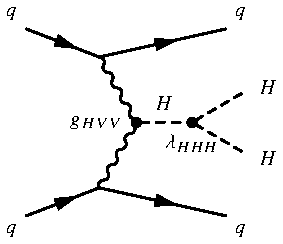
\includegraphics[width=0.3\textwidth]{feynman_graphs/di_higgs_vbf_kvklam}%
      \hfill%
      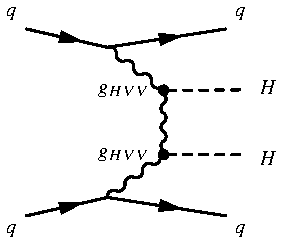
\includegraphics[width=0.3\textwidth]{feynman_graphs/di_higgs_vbf_kvkv}%
      \hfill%
      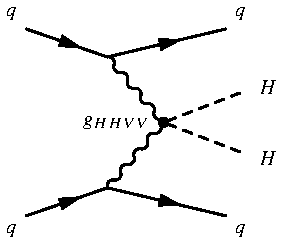
\includegraphics[width=0.3\textwidth]{feynman_graphs/di_higgs_vbf_ktwov}%
      \hspace*{0.04\textwidth}
    \end{minipage}
  }

  \vspace*{1.0em}
  {\scriptsize In $pp$ collisions at $\sqrt{s} = \SI{13}{\TeV}$}
\end{frame}

\begin{frame}{Higgs Boson Pair Production: A Rare Process}

  \begin{columns}
    \column{0.4\textwidth}
    \centering

    % \begin{itemize}
    % \item Total proton--proton collision cross section:\ \SI{80}{\milli\barn}
    % \item W+jets: 20nb
    % \item ttbar: 831.76 pb
    % \item H: 48 pb (ggF) + 4 pb (VBF) (50pb)
    % \item HH: 31.05 + 1.726 = 32.8 fb
    % \item HHH: 80 ab (80e-18)
    % \end{itemize}
    \vspace*{1em} 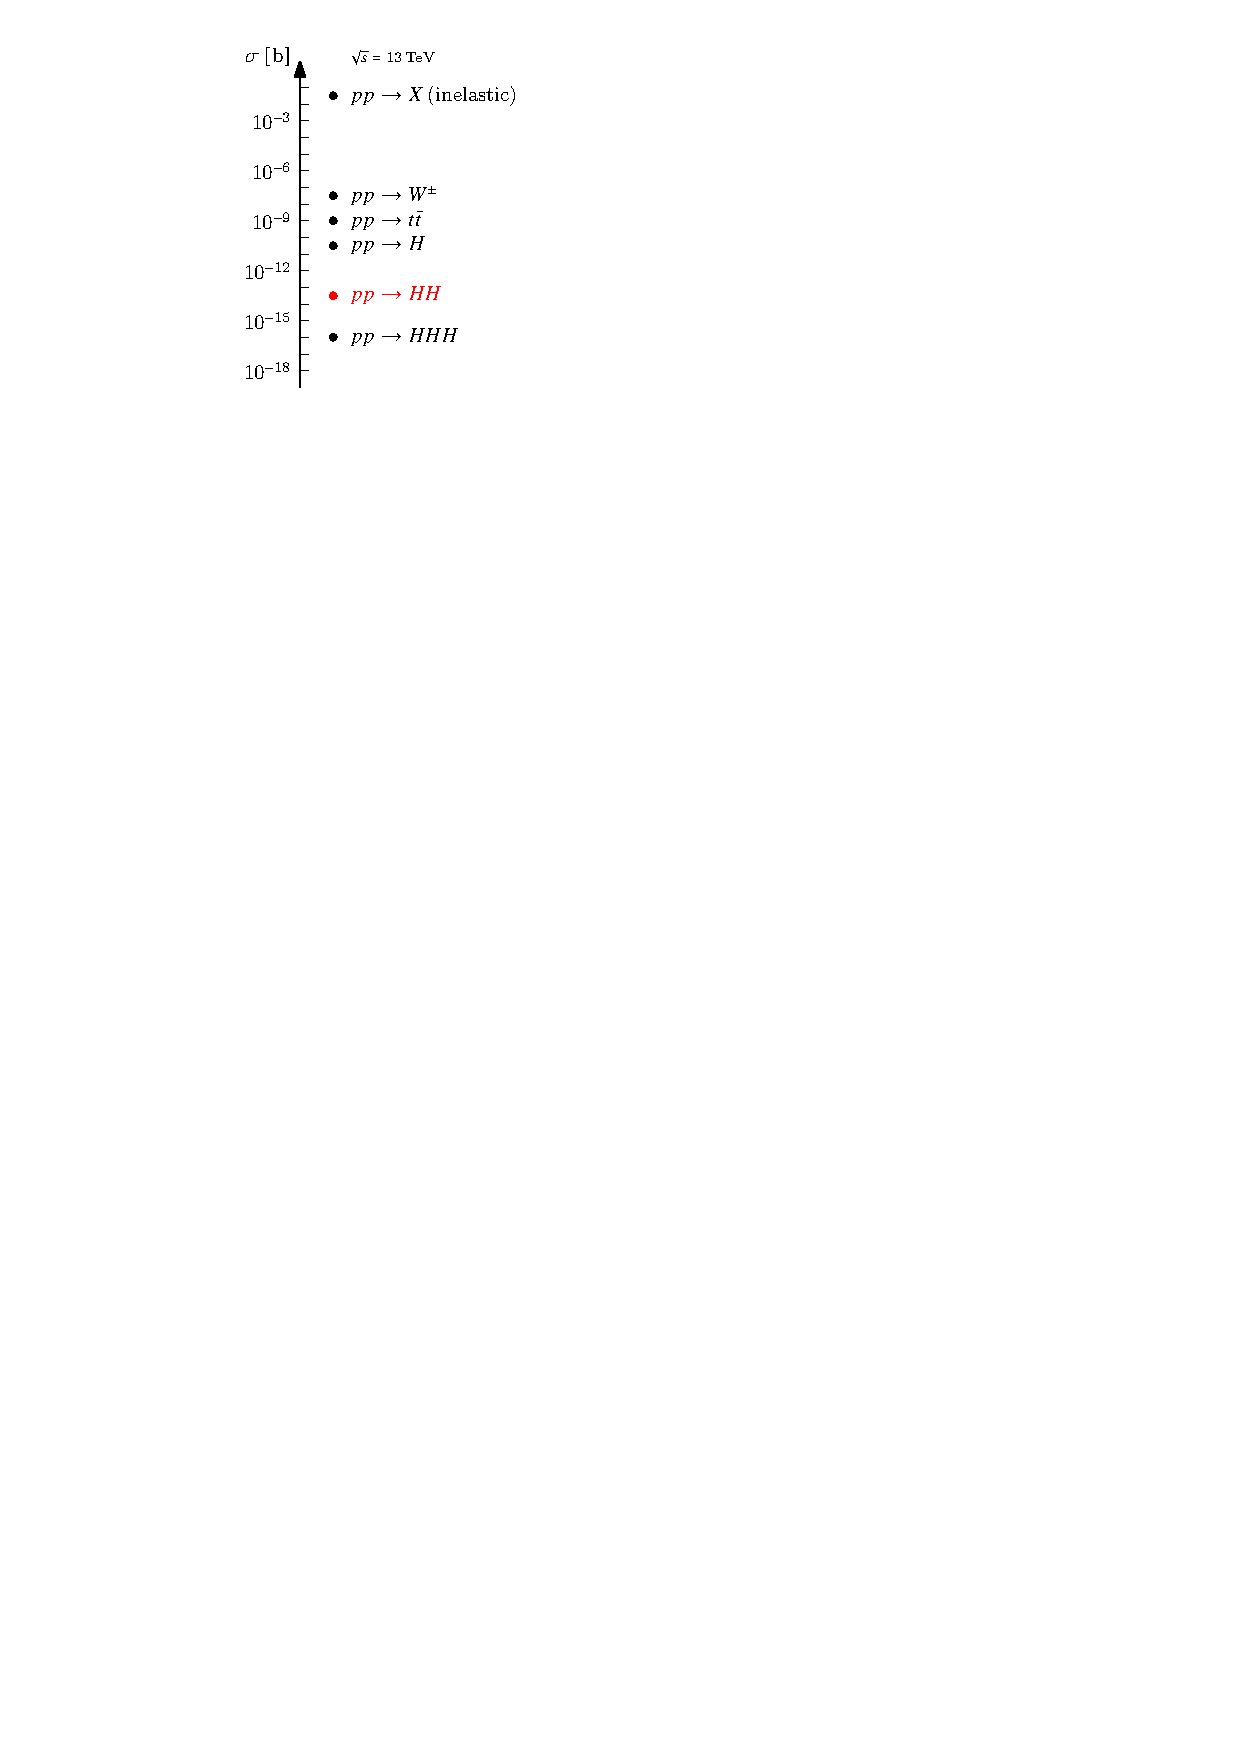
\includegraphics[width=0.92\textwidth]{cross_section_figure}

    \column{0.6\textwidth}

    \textbf{SM Expectation:}
    \vspace{0.5em}
    \begin{itemize}
      \setlength{\itemsep}{1em}

    \item 1 \HH event in 2.5 trillion inelastic collisions

    \item Total of 4000 \HH events produced in ATLAS from 2015--2018

      % Do not expect to find this in Run~2

    \end{itemize}
  \end{columns}
\end{frame}

% ------------------------------------------------------------------------------

\begin{frame}{Beyond the Standard Model}
  \begin{columns}[onlytextwidth]
    \column{0.5\textwidth}

    \textbf{Shortcomings of the SM:}
    \begin{itemize}
    \item Matter--Antimatter Asymmetry
    \item Gravitation
    \item Dark Matter \& Dark Energy
    \item \dots
    \end{itemize}

    \column{0.5\textwidth}

    \hspace*{0.35\textwidth}%
    \begin{overpic}[scale=1,trim=0 0.3cm 0 0, clip]{energy_content/content}
      \put(-70,37){\parbox{1.0in}{\small Energy density of today's universe:}}
      \put(80, 0){\footnotesize Planck 2018}
    \end{overpic}
    % Ordinary matter 4.9 % Dark matter 26.8 % Dark energy 68.3 %
  \end{columns}
  \pause
  \vspace*{1.5em}
  \hrule
  \vspace*{1.5em}
  \begin{columns}
    \column{0.4\textwidth} \centering

    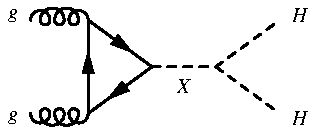
\includegraphics[width=0.8\textwidth]{feynman_graphs/di_higgs_resonant}

    \column{0.6\textwidth}

    \allbold{Search for scalars $X$ decaying to $HH$:}
    \begin{itemize}
      \setlength{\itemsep}{0.5em}
    \item E.g.\ in models with extended Higgs sectors
    \item Mass range:\ $\SI{251}{\GeV} < m_{X} < \SI{1.6}{\TeV}$
    \end{itemize}
  \end{columns}
\end{frame}

% ------------------------------------------------------------------------------

\begin{frame}{The ATLAS Experiment at the LHC}
  \centering
  \includegraphics<1>[scale=0.95]{lhc_atlas/lhc_atlas_1}
  \includegraphics<2>[scale=0.95]{lhc_atlas/lhc_atlas_2}
  % TODO: Add mention of Run~2 and integrated luminosity
\end{frame}

% ------------------------------------------------------------------------------

\begin{frame}{Final States of Searches for \HH Production}
  \begin{columns}[onlytextwidth]
    \column{0.5\textwidth}

    \textbf{Most promising
      channels (SM):}\\
    $b\bar{b}b\bar{b}$, \bbtautau, $b\bar{b}\gamma\gamma$
    \begin{itemize}
    \item Trade-off between branching ratio \& ``cleanliness'' of final state
    \end{itemize}

    \column{0.5\textwidth}
    \centering

    {\small Branching ratios of a $HH$-system:}

    \vspace*{0.5em}

    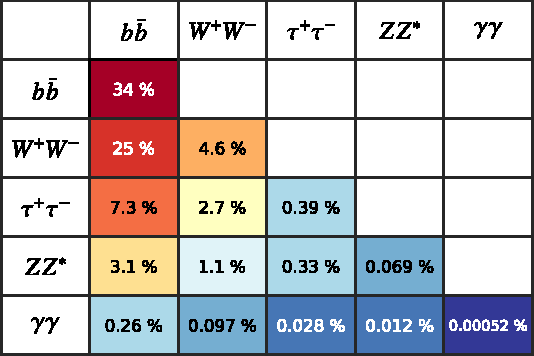
\includegraphics[width=0.9\textwidth]{theory/di_higgs_branching_ratio}
  \end{columns}
\end{frame}

% ------------------------------------------------------------------------------

\begin{frame}{The \bbtautau Final State}

  \begin{columns}[onlytextwidth]
    \column{0.4\textwidth}

    \textbf{Advantages:}
    \begin{itemize}
      \setlength{\itemsep}{0.5em}
    \item Large $H \to b\bar{b}$ branching ratio
    \item Distinct signature of $H \to \tau^+\tau^-$
    \end{itemize}

    \vspace{1em}
    \pause

    \textbf{Channels:}
    \begin{itemize}
      \setlength{\itemsep}{0.5em}
    \item<2-> \lephad channel\\
      $\mathcal{B}(\tau^+\tau^- \to \lephad) \approx \SI{45.6}{\percent}$

    \item<3-> \hadhad channel\\
      $\mathcal{B}(\tau^+\tau^- \to \hadhad) \approx \SI{42.0}{\percent}$
    \end{itemize}

    \column{0.6\textwidth} \centering
    % \begin{overlayarea}{\textwidth}{0.5cm}
    %   \centering
    %   \only<1>{\lephad}%
    %   \only<2>{\hadhad}
    % \end{overlayarea}

    \hspace*{0.03\textwidth}%
    \includegraphics<2>[width=0.97\textwidth]{final_state/final_state_lephad}%
    \includegraphics<3>[width=0.97\textwidth]{final_state/final_state_hadhad}
  \end{columns}
\end{frame}

% ------------------------------------------------------------------------------

\begin{frame}[standout]
  Interlude:\ Tau Identification
\end{frame}

% ------------------------------------------------------------------------------

\begin{frame}{Tau Identification}
  \begin{columns}
    \column{0.45\textwidth} \centering
    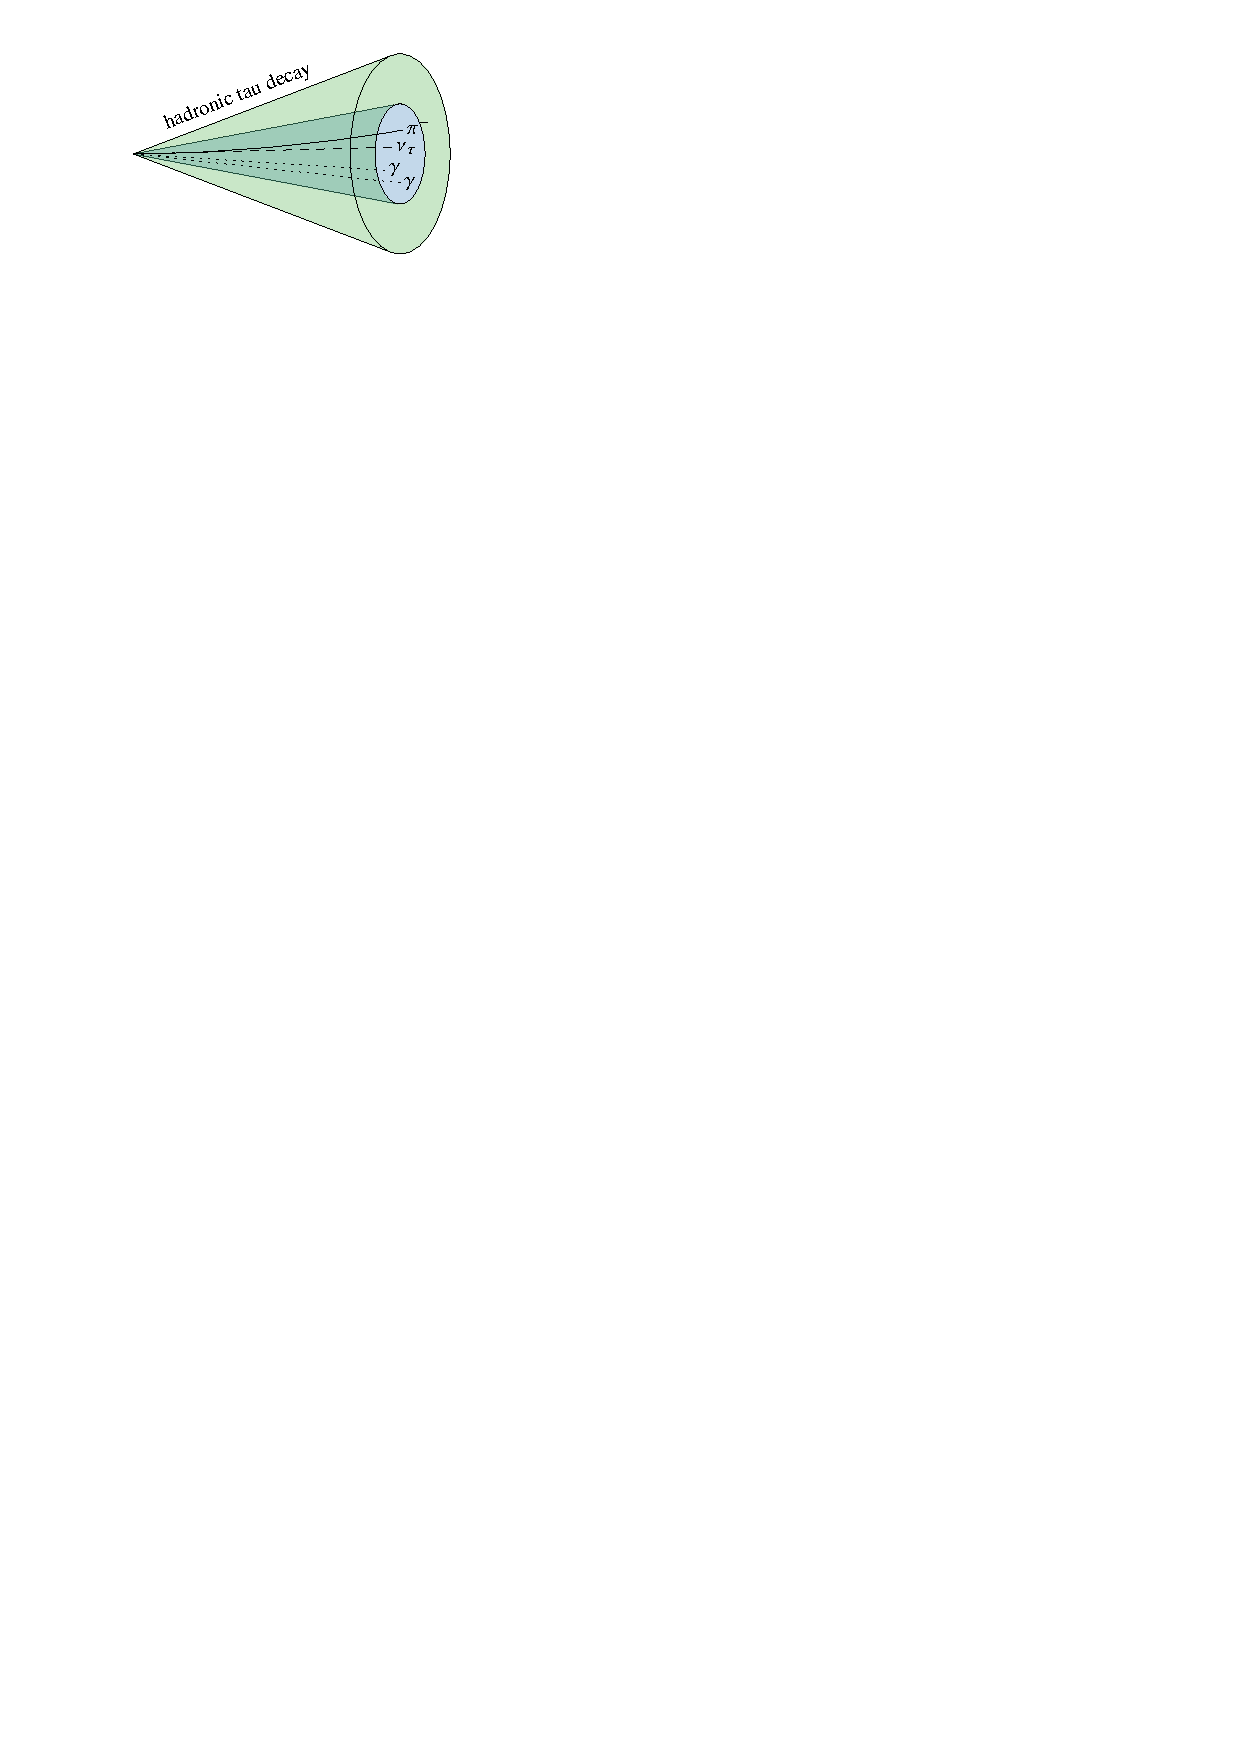
\includegraphics[width=0.75\textwidth]{tauid/cone_tauhad}

    \column{0.10\textwidth}
    \centering

    vs.

    \column{0.45\textwidth}
    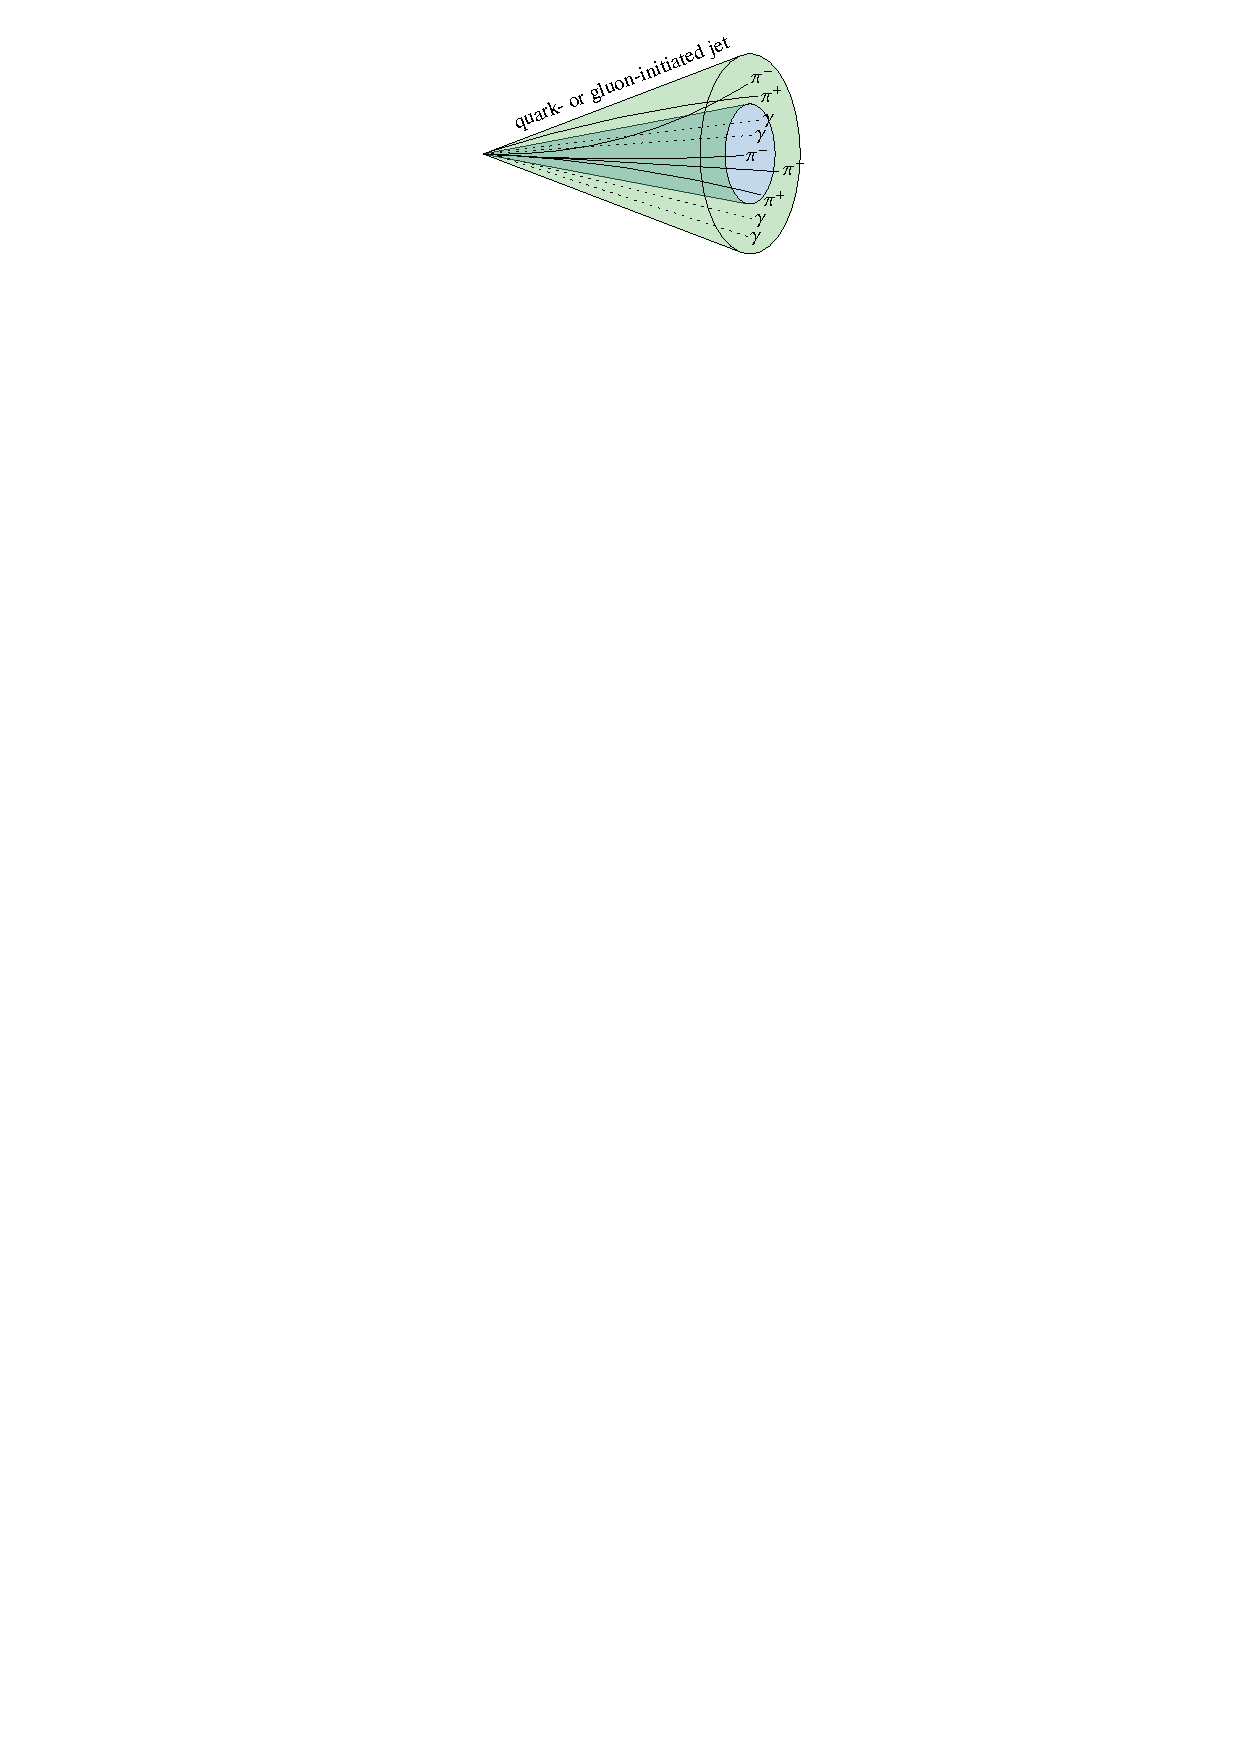
\includegraphics[width=0.75\textwidth]{tauid/cone_qgjet}
  \end{columns}

  \vspace{0.5em}

  \textbf{Characteristic features:}%

  \begin{columns}[onlytextwidth]
    \column{0.5\textwidth}

    \begin{itemize}
    \item Particle multiplicity
    \item $\tau$ lepton mass ($m_\tau \approx \SI{1.78}{\GeV}$)
    \end{itemize}

    \column{0.5\textwidth}

    \begin{itemize}
    \item Isolation
    \item $\tau$ lepton lifetime ($c\tau \approx \SI{87}{\micro\meter}$)
    \end{itemize}
  \end{columns}

  \onslide<2->{%
    \tikz[overlay, remember picture, shift=(current page.south west), x=(current
    page.south east), y=(current page.north west), ]{ \node[align=center] at
      (0.5,0.678) {%
        \setlength{\fboxrule}{1pt}%
        \fcolorbox{headergray}{mygray}{%
          \begin{minipage}{0.75\textwidth}
            \centering \vspace*{0.6em} \textbf{Machine learning techniques}

            Simulated $\gamma^* \rightarrow \tauhad \tauhad$ for ``signal''

            Simulated di-jet events for ``background'' \vspace*{0.6em}
          \end{minipage}
        }
      };
    }
  }
  %     % Optional help grid lines \draw[step=.1, opacity=0.3, thick, red] (0,0)
  %     % grid (1,1); }}
\end{frame}

% ------------------------------------------------------------------------------

% 4. slide: How does it look in the grand scheme?

\begin{frame}{Tau Identification: High-Level Variables}
  \begin{columns}[onlytextwidth]
    \column{0.25\textwidth} \centering

    
\includegraphics[scale=1]{tauid/high_level_icon}

    \column{0.75\textwidth}

    \begin{columns}[onlytextwidth]
      \column{0.5\textwidth}
      \centering

      $p_{\text{T}}$-fraction of \emph{isolation} tracks\\[0.2em]

      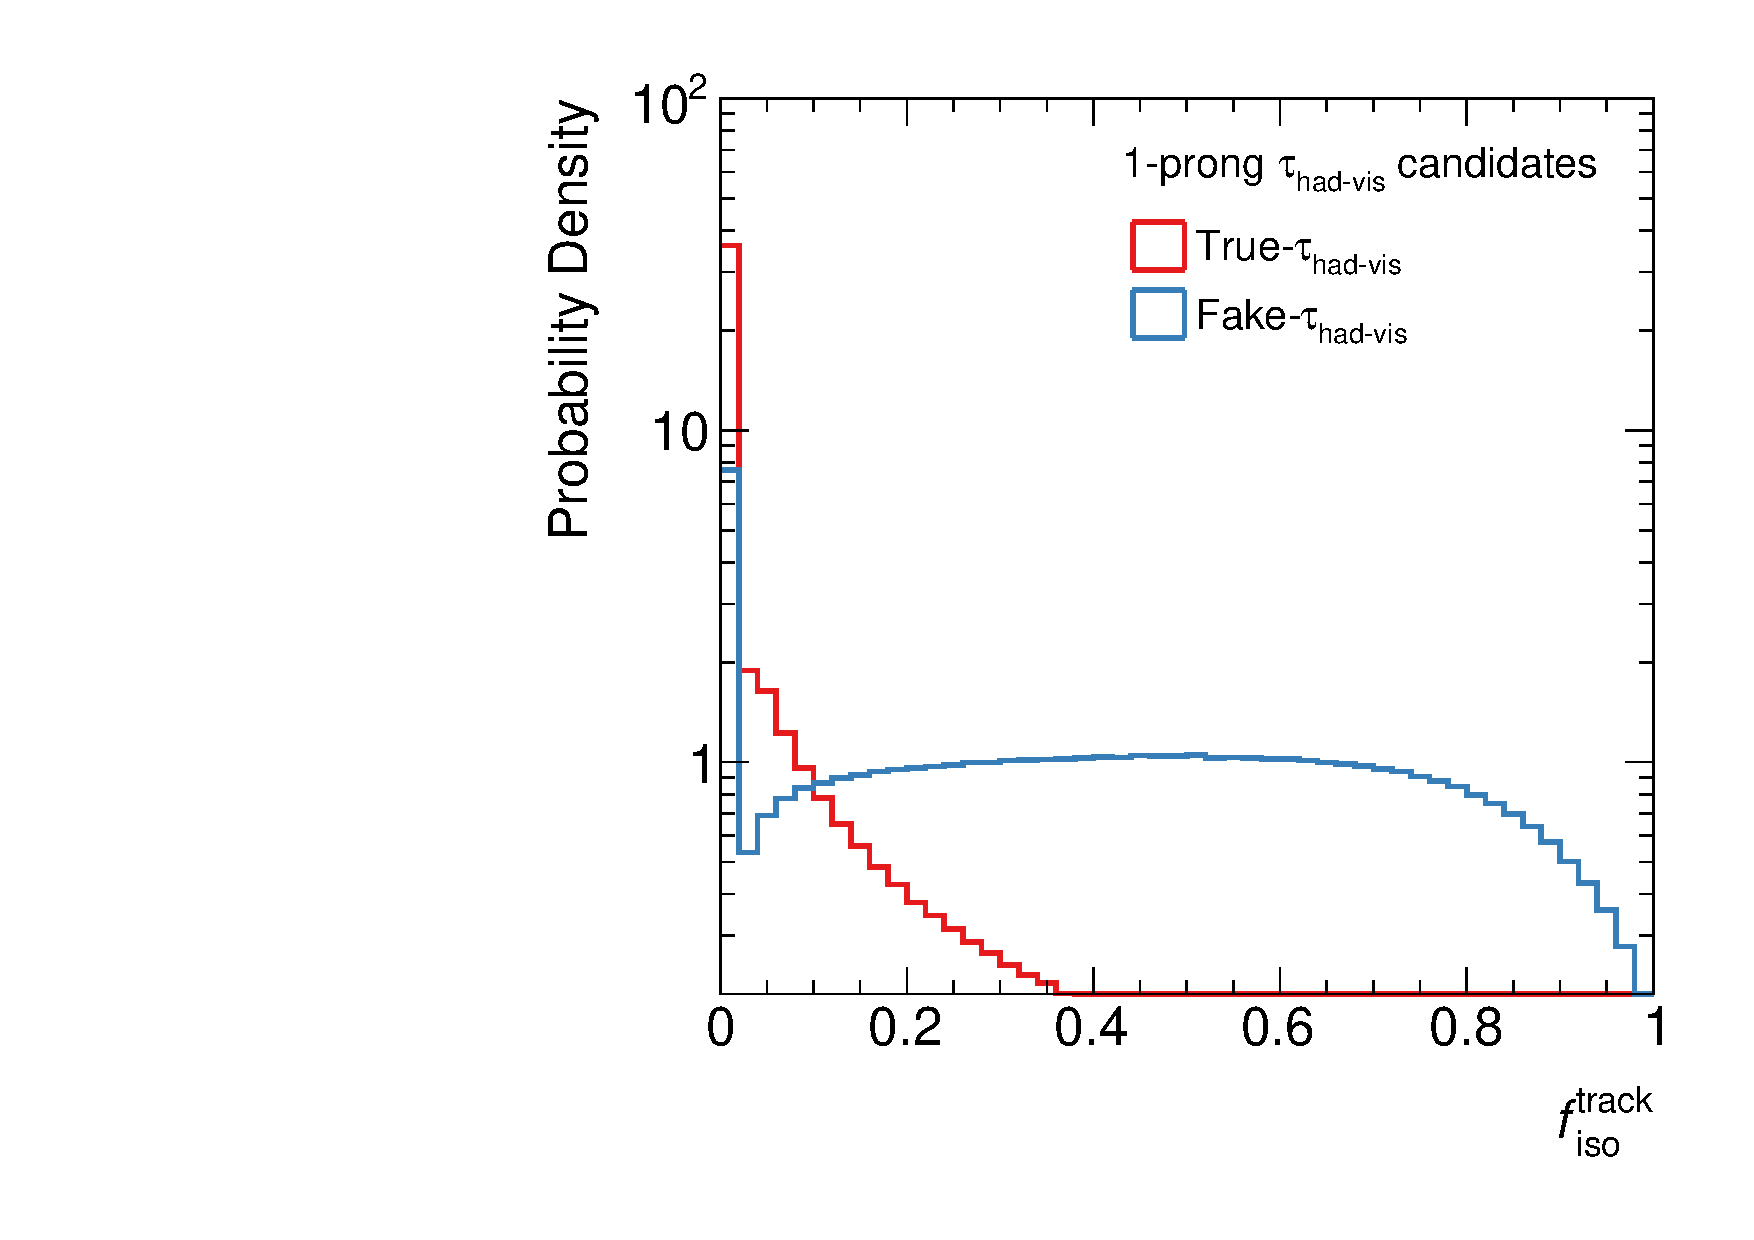
\includegraphics[width=0.9\textwidth]{tauid/invars/invars_sumpttrkfrac_1P}

      \column{0.5\textwidth}
      \centering

      \only{Invariant mass of \emph{core} tracks\\[0.2em]}

      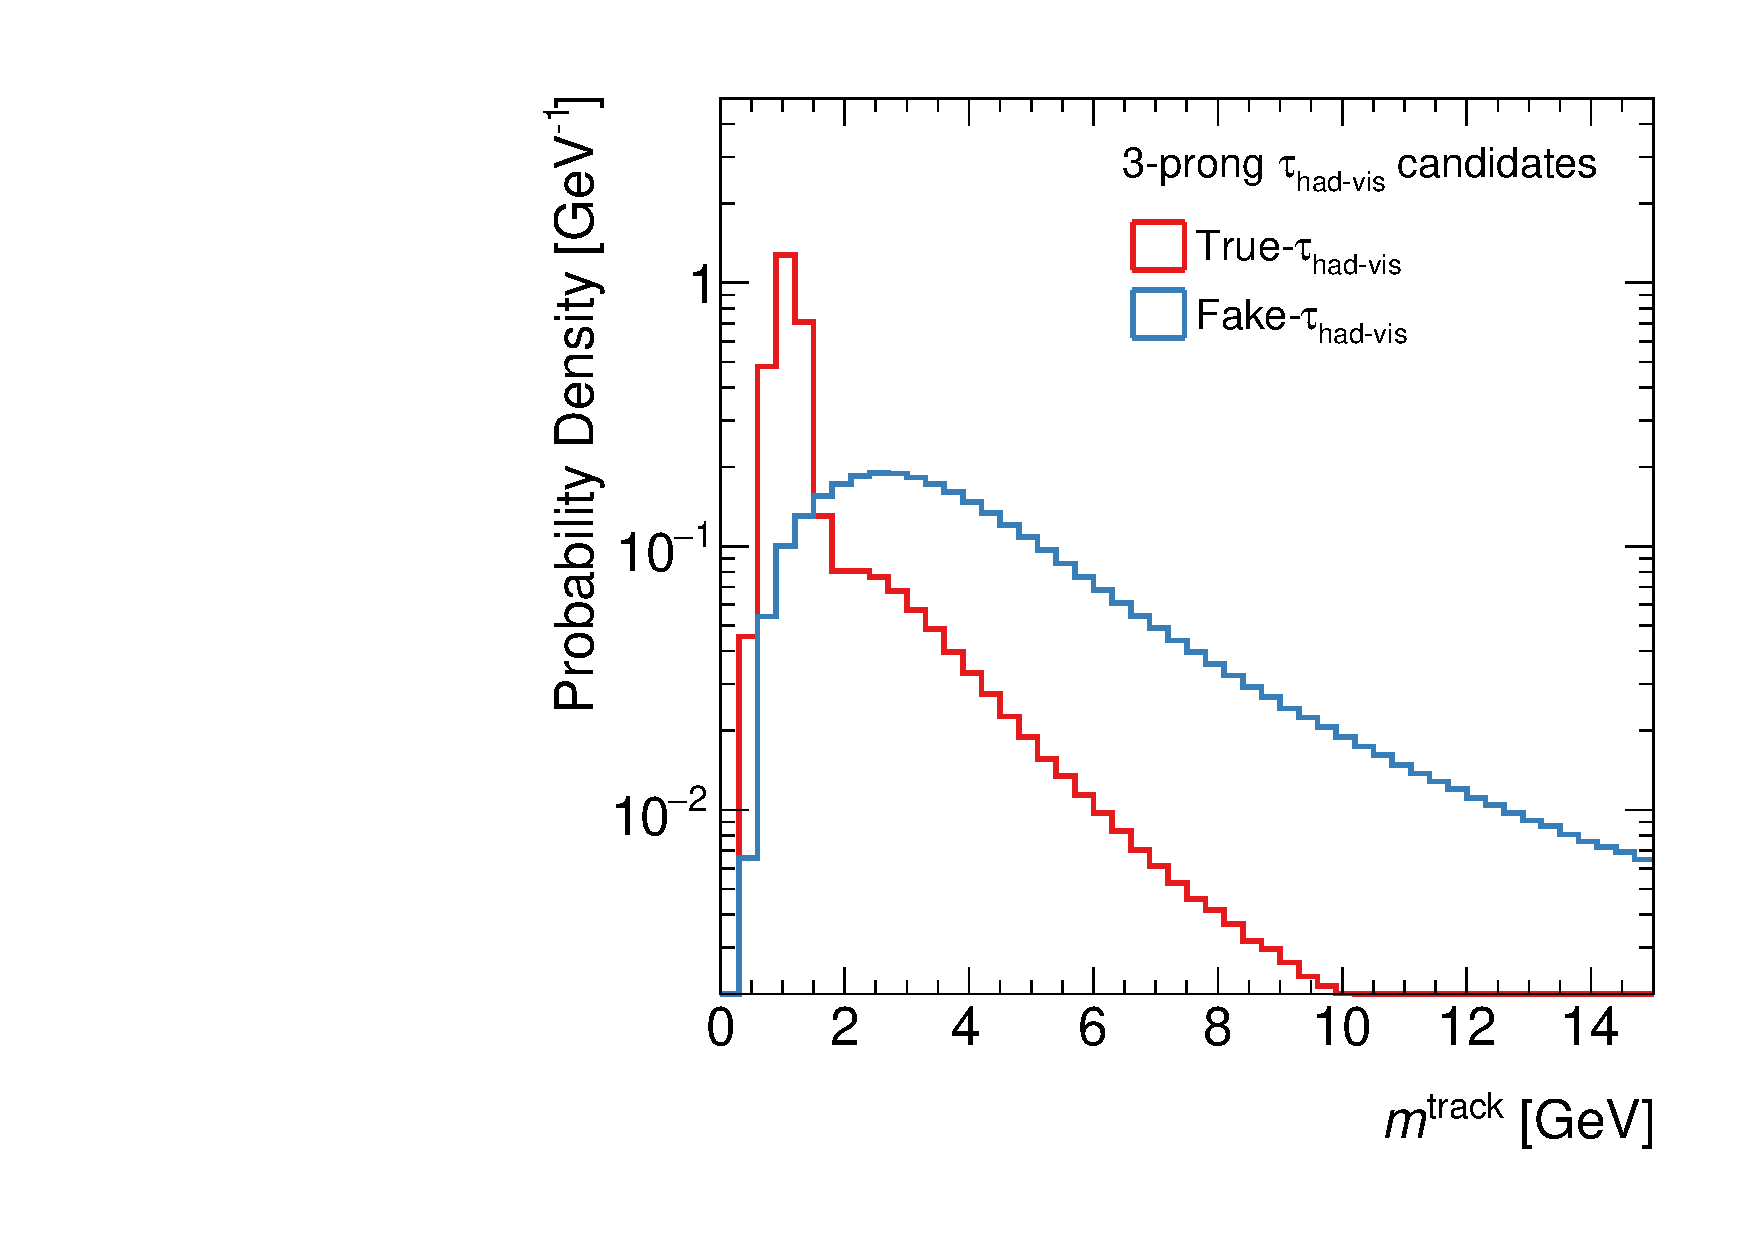
\includegraphics[width=0.9\textwidth]{tauid/invars/invars_masstrksys_3P}
    \end{columns}

    \vspace*{0.5em}

    \begin{itemize}
    \item Total 11 discriminating variables considered
    \item Previously used in \emph{Boosted Decision Trees} (BDTs) for Tau-ID
    \end{itemize}
  \end{columns}
\end{frame}

% ------------------------------------------------------------------------------

\begin{frame}{Previous Tau Identification Approach}
    \begin{center}
    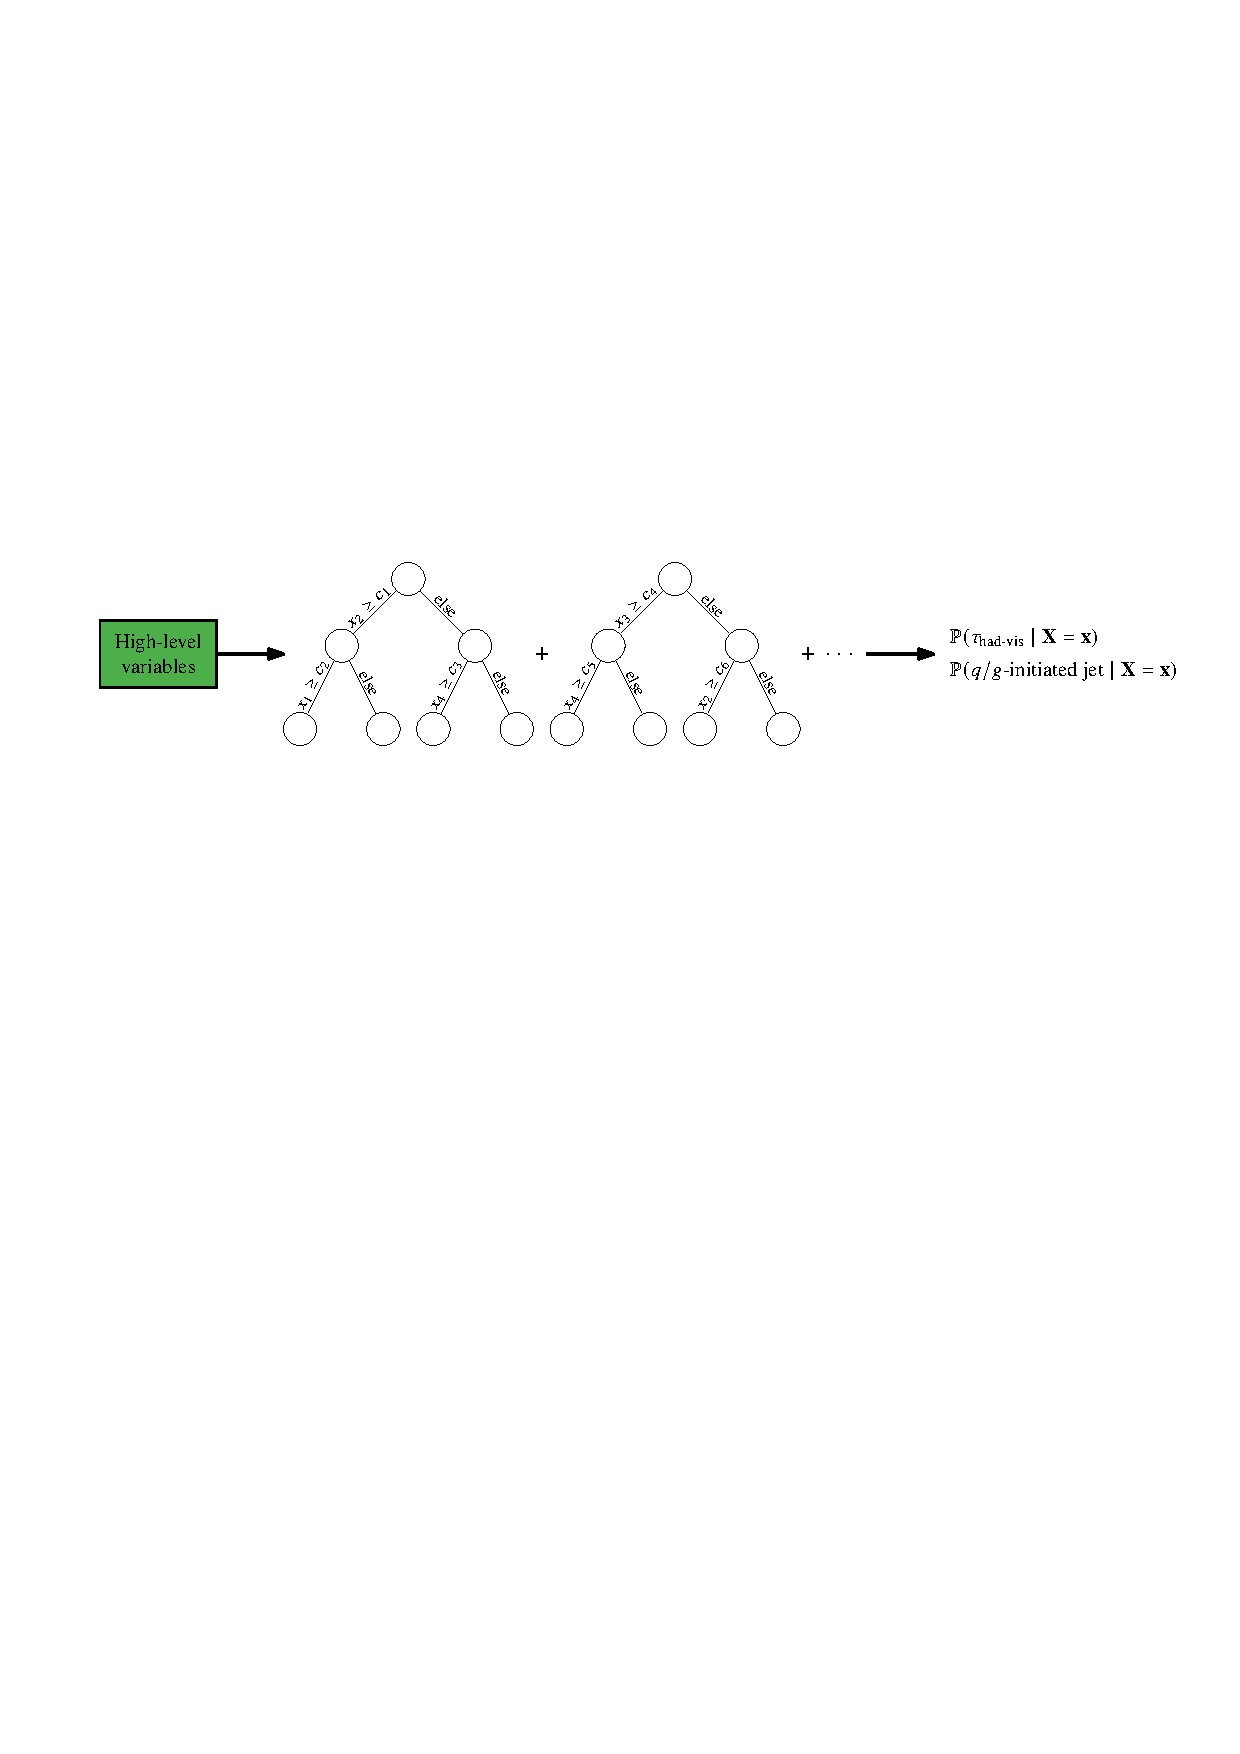
\includegraphics[scale=0.75]{tauid/bdt_approach}
  \end{center}

  Using Boosted Decision Trees.
\end{frame}

% ------------------------------------------------------------------------------

\begin{frame}{Tau Identification with RNN}
  \begin{columns}[onlytextwidth]
    \column{0.25\textwidth} \centering

    
\includegraphics[scale=1]{tauid/track_icon}

    \column{0.75\textwidth}

    {\centering
      $p_{\text{T}}$ of leading and sub-leading track\\[0.17em]
    }

    \begin{columns}[onlytextwidth]
      \column{0.5\textwidth} \centering

      \includegraphics<1>[width=0.9\textwidth]{tauid/invars/invars_trk0relpt_1P}

      \column{0.5\textwidth}
      \centering

      \includegraphics<1>[width=0.9\textwidth]{tauid/invars/invars_trk1relpt_1P}
    \end{columns}

    \vspace*{0.5em}

    \begin{itemize}
    \item Up to 10 tracks within $\Delta R < 0.4$ of tau axis
    \item
    \end{itemize}
  \end{columns}
\end{frame}

% ------------------------------------------------------------------------------

\begin{frame}{Tau Identification with RNN}
  \begin{columns}[onlytextwidth]
    \column{0.25\textwidth} \centering

    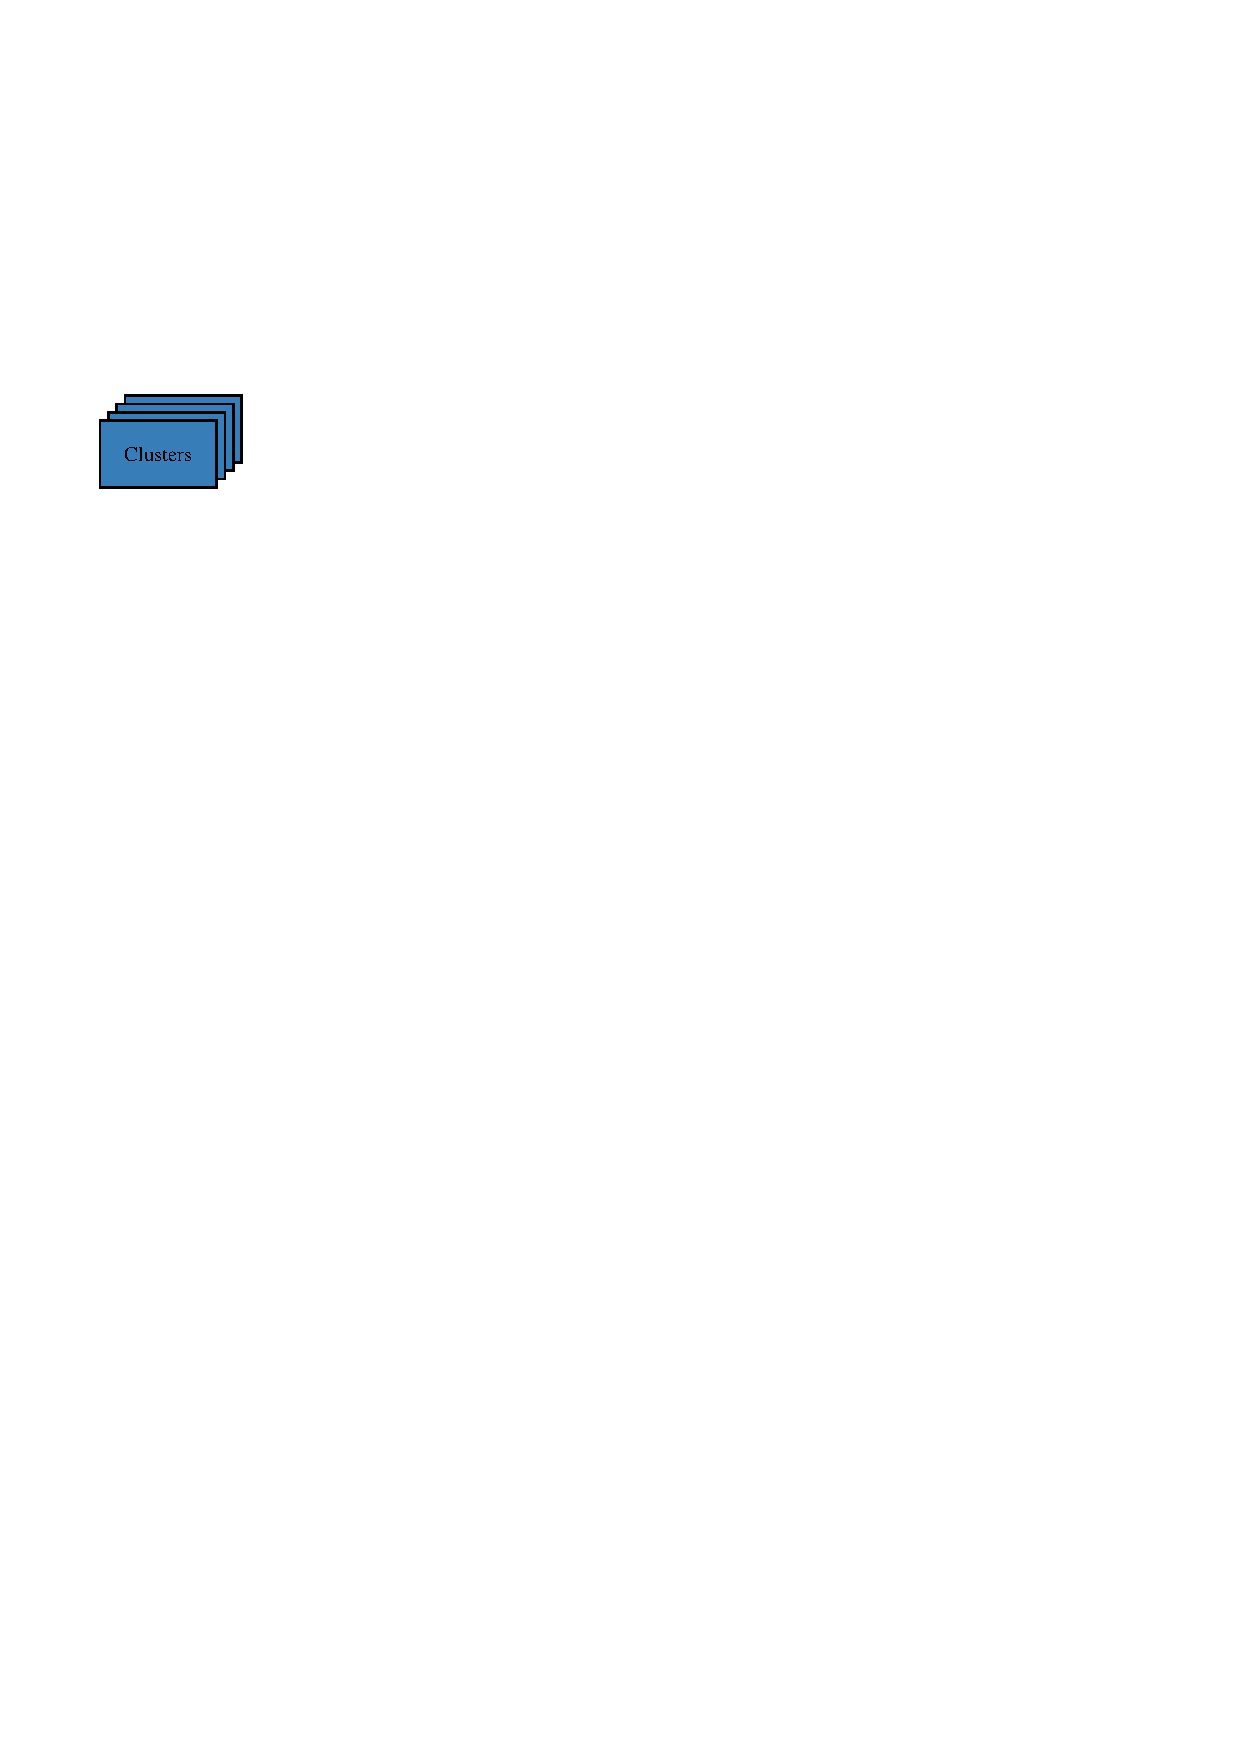
\includegraphics[scale=1]{tauid/cluster_icon}

    \column{0.75\textwidth}

    {\centering
      $E_{\text{T}}$ of leading and sub-leading cluster\\[0.17em]
    }

    \begin{columns}[onlytextwidth]
      \column{0.5\textwidth} \centering

      \includegraphics<1>[width=0.9\textwidth]{tauid/invars/invars_cls0relet_3P}

      \column{0.5\textwidth}
      \centering

      \includegraphics<1>[width=0.9\textwidth]{tauid/invars/invars_cls1relet_3P}
    \end{columns}

    \vspace*{0.5em}

    \begin{itemize}
    \item Up to 6 clusters associated to the jet seed
    \item
    \end{itemize}
  \end{columns}
\end{frame}

% ------------------------------------------------------------------------------

\begin{frame}{Approach}

  \textbf{New method based on Recurrent Neural Networks:}\\[0.5em]
  \begin{center}
    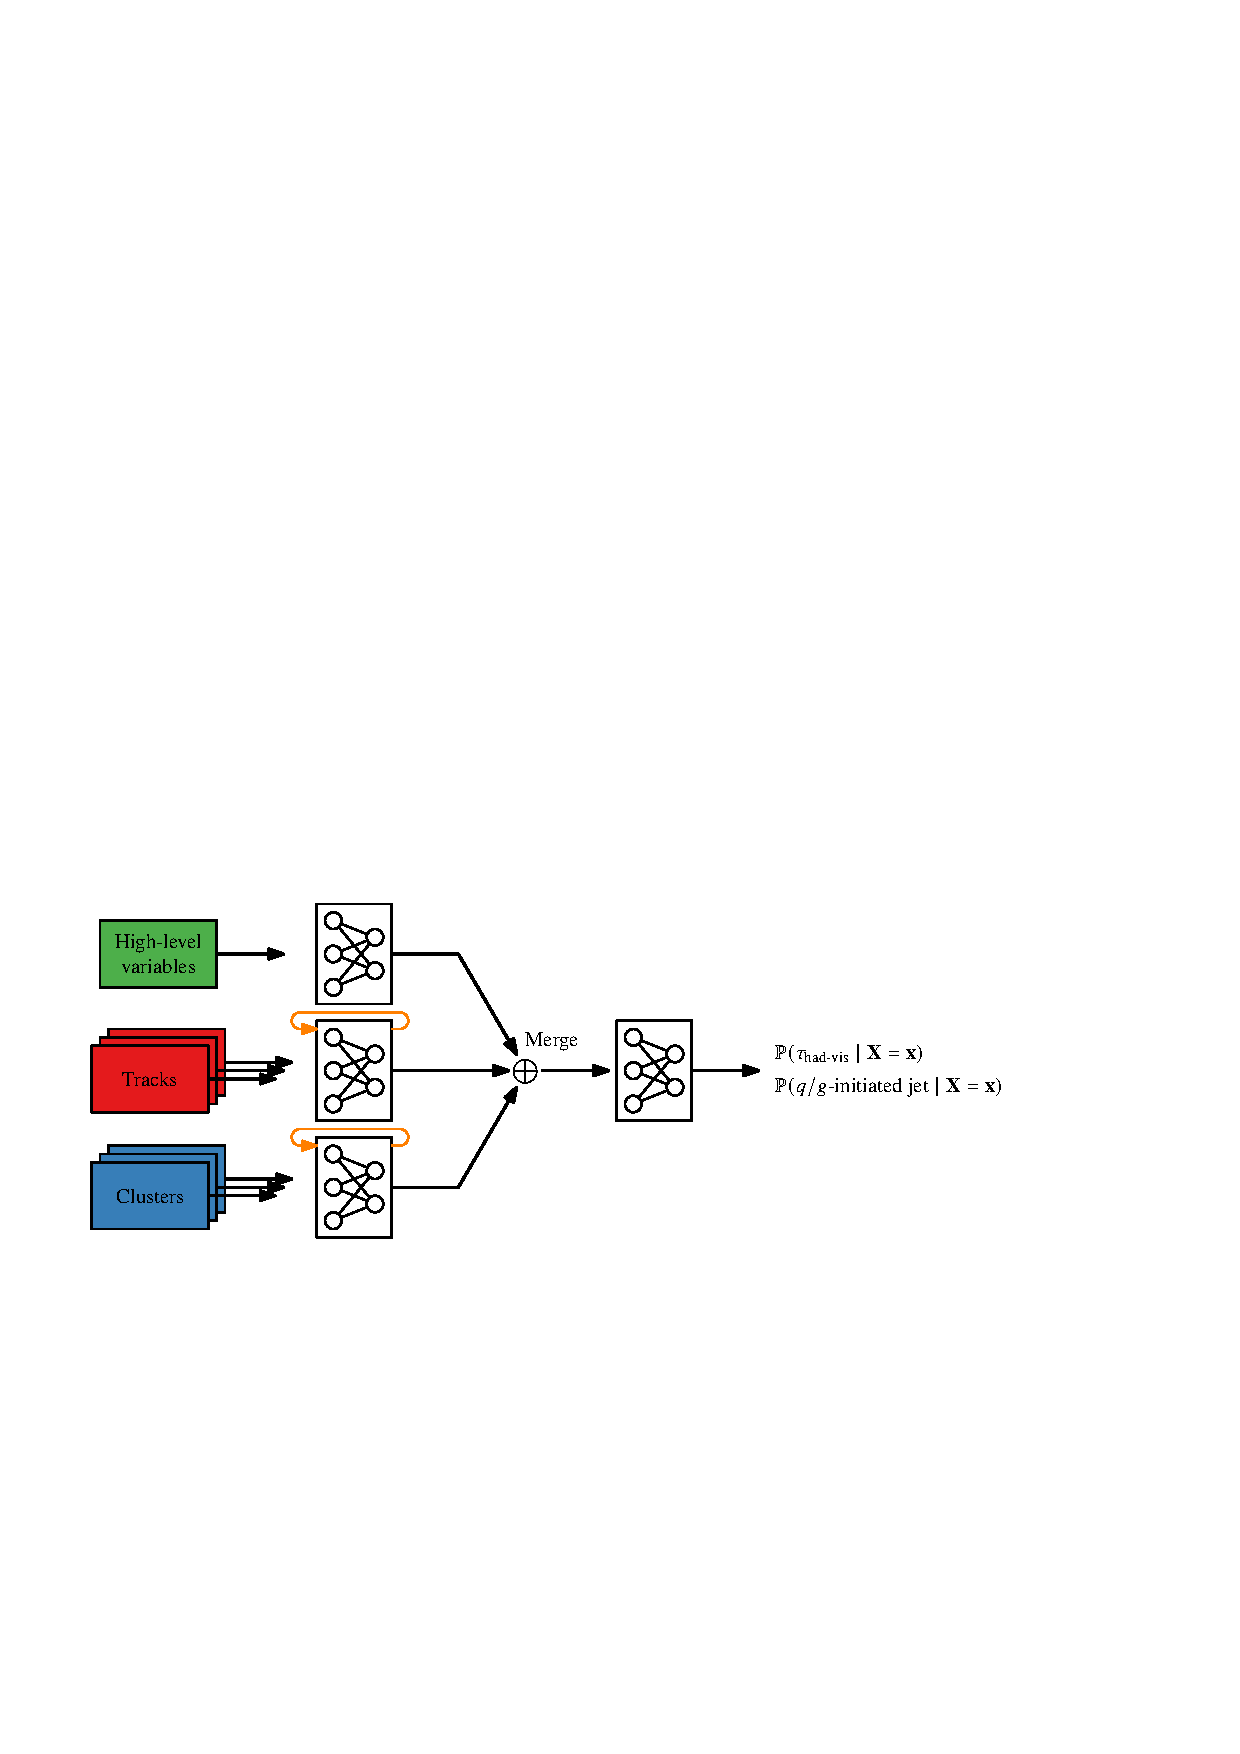
\includegraphics[scale=0.75]{tauid/rnn_approach}
  \end{center}
\end{frame}

% ------------------------------------------------------------------------------

\begin{frame}{Performance of RNN-Based Tau Identification}

  \begin{columns}[onlytextwidth]
    \column{0.5\textwidth}
    \begin{itemize}
    \item Four working points:\\
      \emph{Very Loose}, \emph{Loose}, \emph{Medium}, \emph{Tight}

      % \item Adopted for offline reconstruction and at the high-level trigger

    \end{itemize}


    \begin{center}
      \footnotesize
      \begin{tabular}{lcc}
        \toprule
        & \multicolumn{2}{c}{Rejection Improvement}\\
        WP & 1-prong \tauhadvis & 3-prong \tauhadvis \\
        \midrule
        Very Loose & +85\,\% & +40\,\% \\
        Loose      & +75\,\% & +50\,\% \\
        Medium     & +80\,\% & +60\,\% \\
        Tight      & +80\,\% & +80\,\% \\
        \bottomrule
      \end{tabular}
    \end{center}

    \column{0.5\textwidth}
    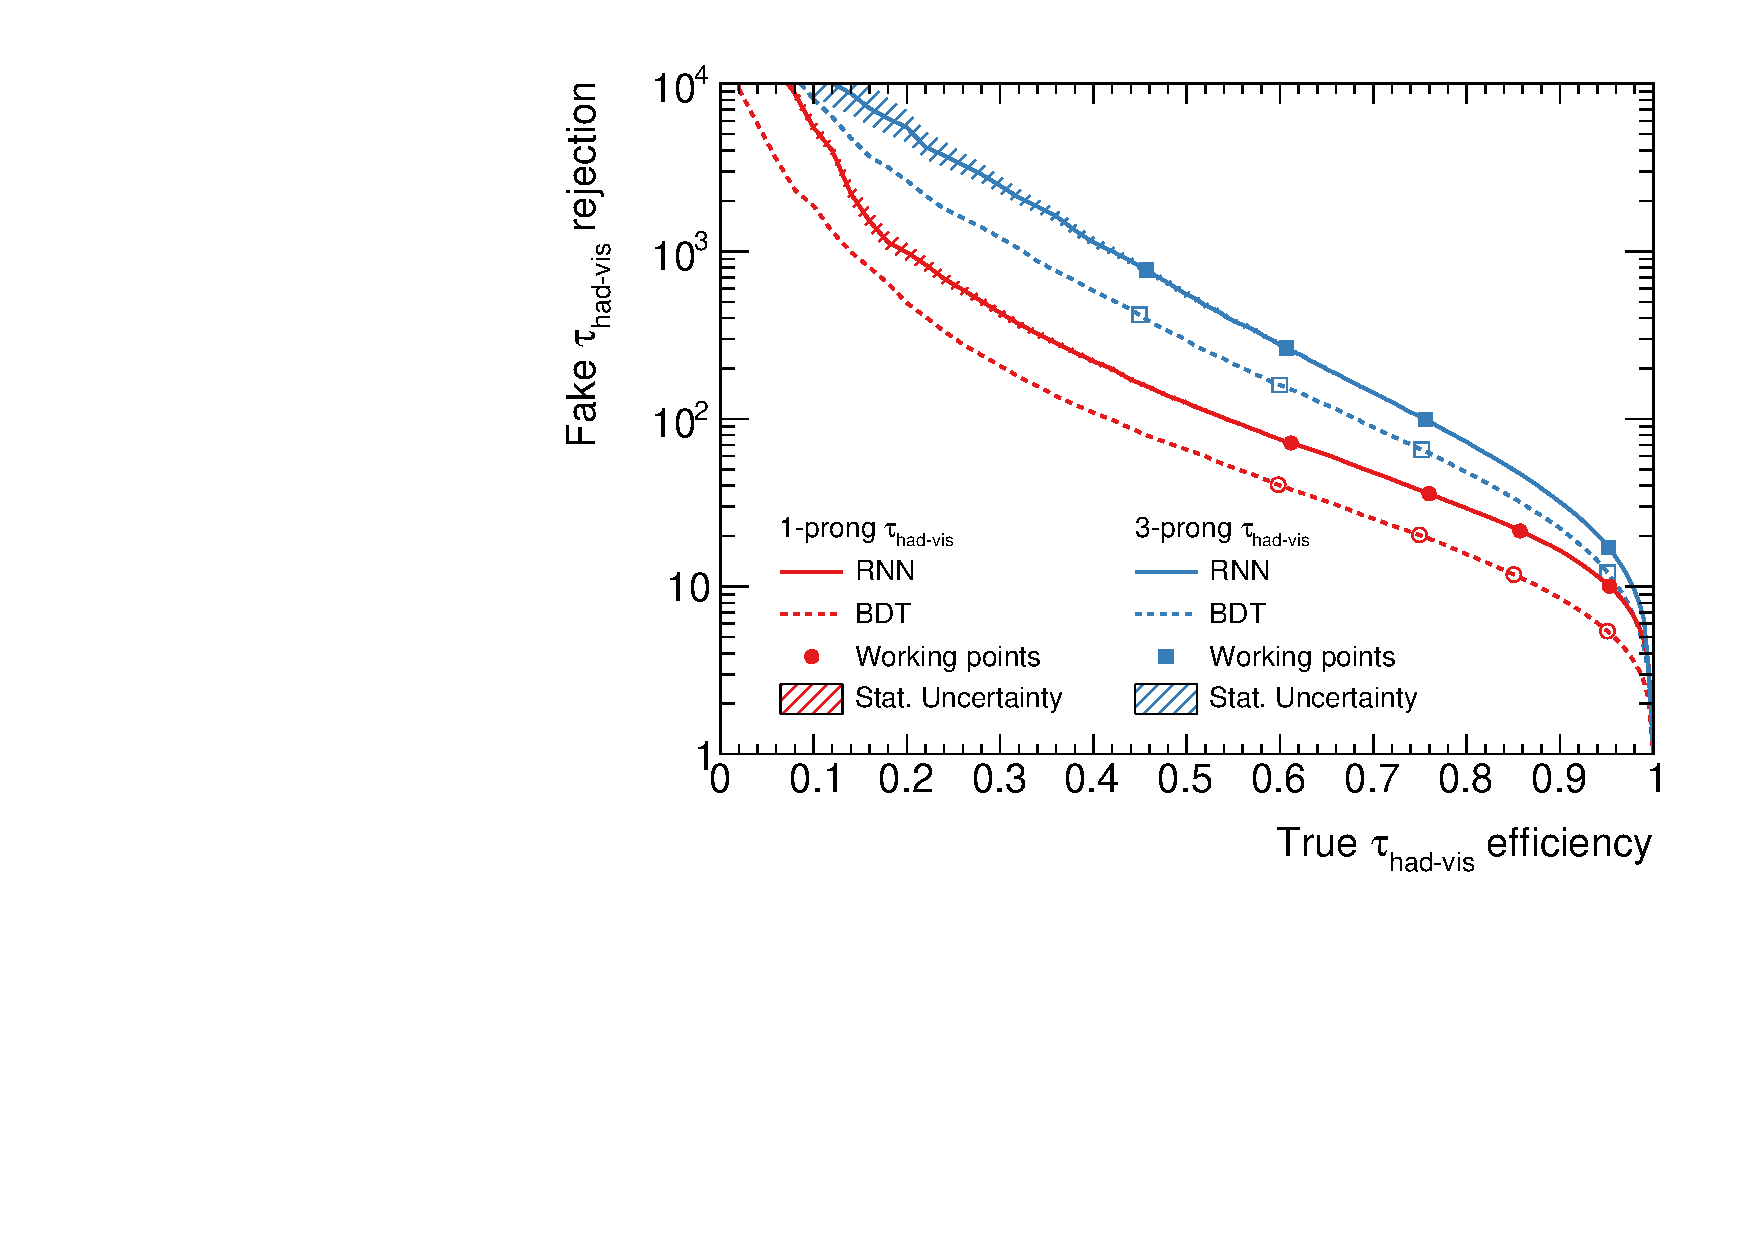
\includegraphics[width=1.0\textwidth]{tauid/roc_incl_witherrors}
  \end{columns}
\end{frame}

% ------------------------------------------------------------------------------

\begin{frame}[standout]
  Back to $HH \rightarrow \bbtautau$
\end{frame}

% ------------------------------------------------------------------------------

\begin{frame}{Object Selection}
  \begin{columns}[onlytextwidth]
    \column{0.5\textwidth}

    \allbold{Electrons/Muons:}
    \begin{itemize}
    \item $\pT > \SI{7}{\GeV}$
    \item Loose identification \& isolation
    \end{itemize}

    \vspace*{1em}

    \allbold{\tauhadvis:}
    \begin{itemize}
    \item $\pT > \SI{20}{\GeV}$
    \item Loose RNN Tau-ID
    \item Electron veto
    \end{itemize}

    \column{0.5\textwidth}

    \allbold{Jets:}
    \begin{itemize}
    \item Anti-$k_{t}$ ($R = 0.4$) particle flow jets
    \item Jet Vertex Tagger
    \item $\pT > \num{20} \, (\num{30})\,\si{\GeV}$ (forward jets)
    \item $b$-tagging with \textsc{DL1r} (\SI{77}{\percent} WP)
    \end{itemize}

    \vspace*{1em}

    \allbold{\pTmissAbs:}
    \begin{itemize}
    \item Object-based with track soft term
    \end{itemize}
  \end{columns}

  % Mention OLR?
\end{frame}

% ------------------------------------------------------------------------------

\begin{frame}{Event Selection}
  % TODO: Tightened ID requirements for leptons in lephad
  \begin{center}
    \footnotesize

    \begin{tabular}{c@{\hskip 2em}c@{\hskip 3em}c}
      \toprule
      \textcolor{hhblue}{\hadhad} & \textcolor{lhred}{\lephad (SLT)} & \textcolor{lhred}{\lephad (LTT)} \\
      \midrule
      \textcolor{hhblue}{single- \& di-\tauhadvis triggers} & \textcolor{lhred}{single-$\ell$ triggers} & \textcolor{lhred}{$\ell+\tauhadvis$ triggers} \\
      \textcolor{hhblue}{exactly two $\tauhadvis$} & \multicolumn{2}{c}{\textcolor{lhred}{exactly one $\tauhadvis$}} \\
      \textcolor{hhblue}{no loose $e$ or $\mu$} & \multicolumn{2}{c}{\textcolor{lhred}{exactly one tight $e$ or medium $\mu$}} \\
                                  & \multicolumn{2}{c}{\textcolor{lhred}{$m_{bb} < \SI{150}{\GeV}$}} \\
      \midrule
      \multicolumn{3}{c}{trigger-dependent thresholds on $e$/$\mu$/$\tauhad$ and jets} \\
      \multicolumn{3}{c}{$m_{\tau\tau}^\text{MMC} > \SI{60}{\GeV}$} \\
      \multicolumn{3}{c}{2 $b$-tagged jets} \\
      \multicolumn{3}{c}{OS electric charge of $e / \mu / \tauhad$ and \tauhad} \\
      \bottomrule
    \end{tabular}
  \end{center}

  % \begin{minipage}[c]{0.45\textwidth}
  %   \centering
  %   \small

  %   Acceptance of non-res.\ $HH$ (SM):

  %   \vspace{1em}

  %   \begin{tabular}{lc}
  %     \toprule
  %     Channel & $(\mathcal{A} \times \varepsilon)^\text{ggF+VBF}_{\text{SM } HH}$ \\
  %     \midrule
  %     \hadhad & 4.0\,\% \\
  %     \lephad (SLT) & 4.0\,\% \\
  %     \lephad (LTT) & 0.97\,\% \\
  %     \bottomrule
  %   \end{tabular}
  % \end{minipage}%
  % \begin{minipage}[c]{0.55\textwidth}
  %   \centering
  %   \small

  %   %Acceptance of narrow scalar resonances:

  %   %\vspace{0.4em}

  %   \begin{overpic}[width=0.9\textwidth]{selection/acceptance_resonant}
  %     %\put(54.5,68){\scriptsize ATLAS-CONF-2021-030}
  %   \end{overpic}
  % \end{minipage}

  % \onslide<2->{
  %   \tikz[overlay, remember picture,
  %   shift=(current page.south west),
  %   x=(current page.south east), y=(current page.north west),
  %   ]{
  %     \node[align=center]at (0.5,0.678) {
  %       \setlength{\fboxrule}{1pt}
  %       \fcolorbox{headergray}{mygray}{%
  %         \begin{minipage}{0.75\textwidth}
  %           \vspace*{0.6em}
  %           \begin{itemize}
  %             \setlength{\itemsep}{1em}
  %           \item Close to \alert{two-fold improvement in signal acceptance} compared to previous publication\\
  %             {\scriptsize (Phys. Rev. Lett. \textbf{121}, 191801)}

  %           \item Driven by \alert{improved reconstruction and identification
  %             of $\tauhad$ and $b$-jets}\\
  %             {\scriptsize (ATL-PHYS-PUB-2017-003, ATL-PHYS-PUB-2017-013, ATL-PHYS-PUB-2019-033)}

  %           \end{itemize}
  %           \vspace*{0.8em}
  %         \end{minipage}
  %       }
  %     };
  %     % Optional help grid lines
  %     % \draw[step=.1, opacity=0.3, thick, red] (0,0) grid (1,1);
  % } }
\end{frame}

% ------------------------------------------------------------------------------
\begin{frame}{Signal Acceptance}

  \vspace*{-1em}

  \begin{columns}[onlytextwidth, t]
    \column{0.5\textwidth}
    \centering

    \allbold{Non-resonant $HH$ production (SM)}

    \vspace{1.5em}

    \resizebox{1.0\textwidth}{!}{\footnotesize
      \begin{tabular}{lcc}
        \toprule
        & \allbold{This Analysis} & Prev.\ Publication \\
        \cmidrule{2-3}
        Channel & $(\mathcal{A} \times \varepsilon)^{gg\text{F+VBF}}_{\text{SM } HH}$ & $(\mathcal{A} \times \varepsilon)^{gg\text{F}}_{\text{SM } HH}$ \\
        \midrule
        \hadhad & 4.0\,\%\phantom{7} & 1.9\,\% \\
        \lephad (SLT) & 4.0\,\%\phantom{7} & \multirow{2}{*}{\hspace*{-1.05em}\bigg\} 3.2\,\%}\\
        \lephad (LTT) & 0.97\,\% & \\
        \bottomrule
      \end{tabular}
    }

    \column{0.5\textwidth}
    \centering

    \allbold{Resonant $HH$ production}

    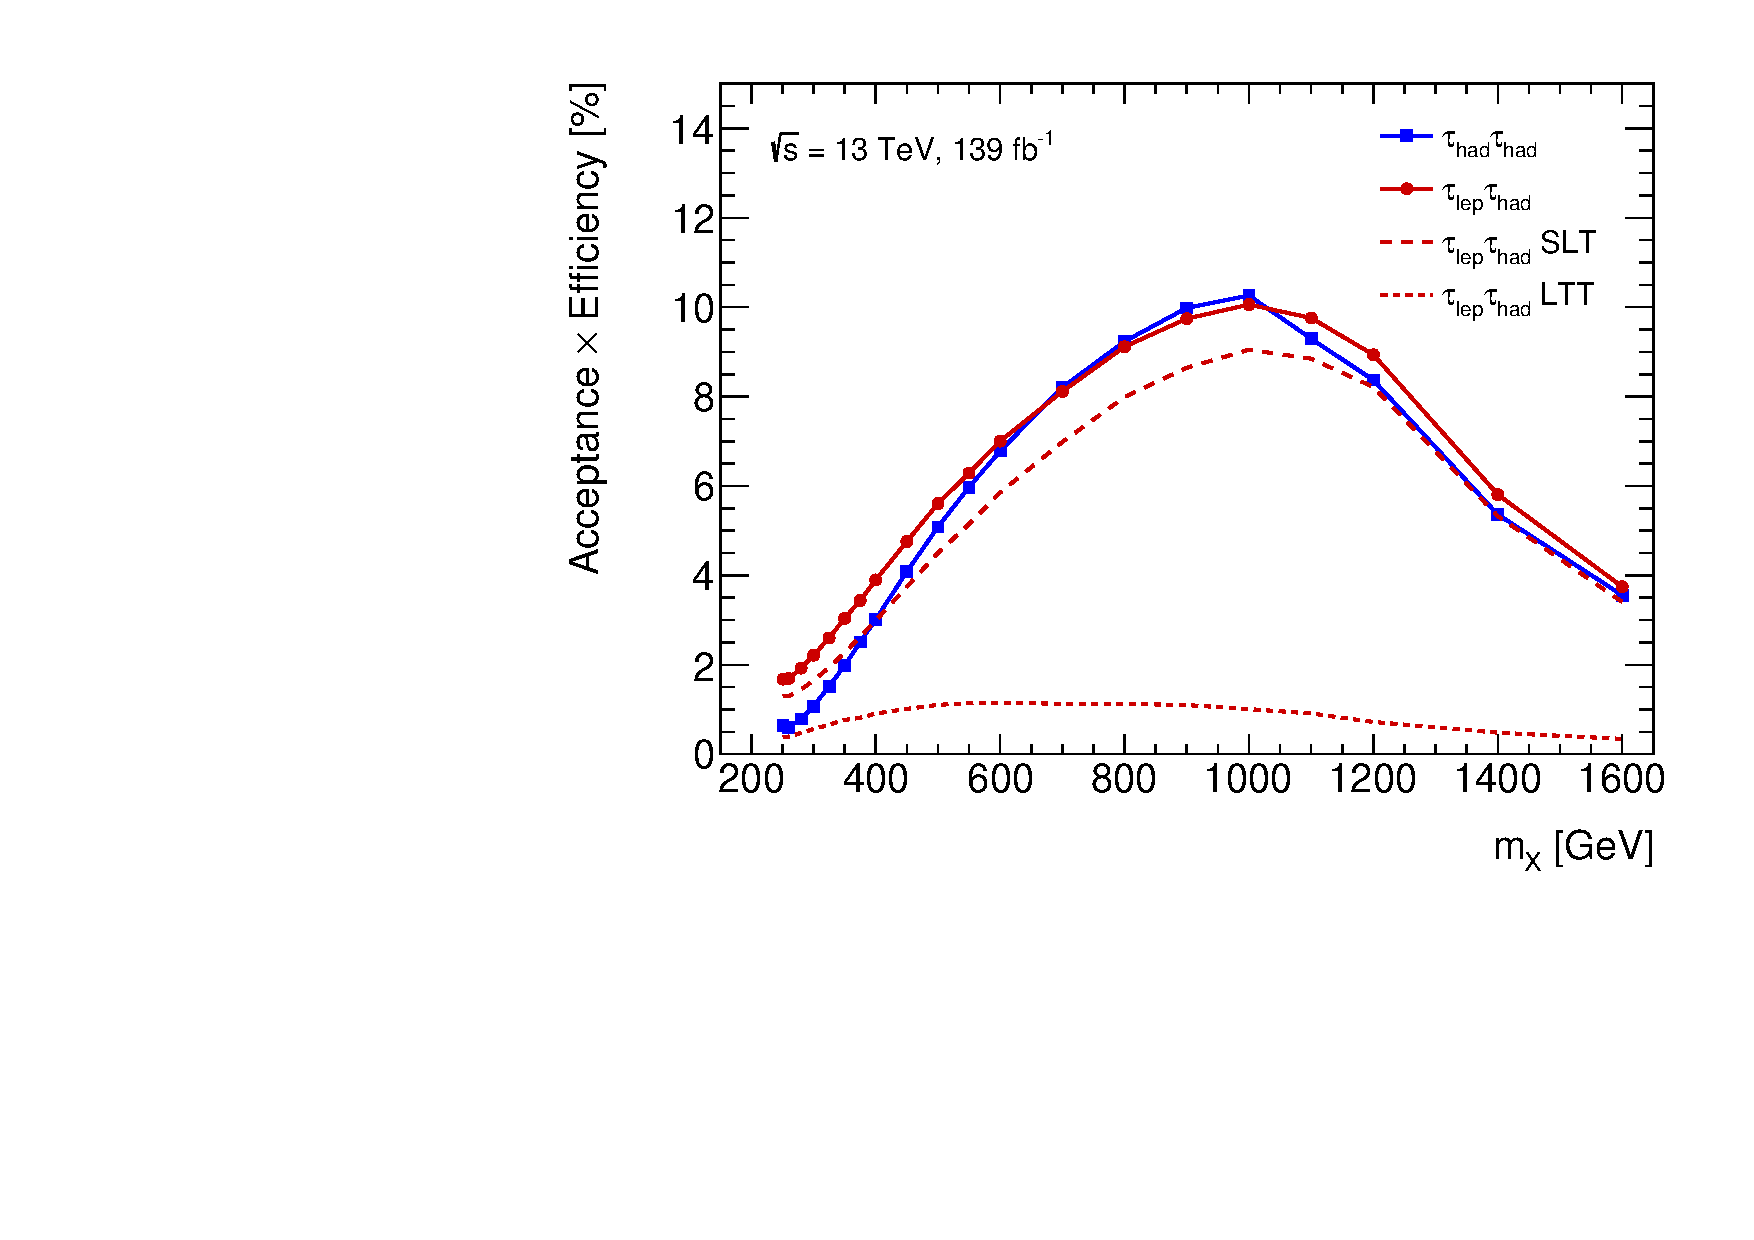
\includegraphics[width=0.8\textwidth]{selection/acceptance_resonant}
  \end{columns}

  \alert{Signal acceptance improvement of \SIrange{50}{100}{\percent}} compared
  to previous publication {\scriptsize (Phys.~Rev.~Lett.~\textbf{121},~191801)}
  \begin{itemize}

  \item Due to improved reconstruction and identification techniques for
    \tauhadvis and $b$-jets

  \end{itemize}
\end{frame}

% ------------------------------------------------------------------------------

\begin{frame}{Background Estimation: Overview}
    \begin{minipage}{0.5\textwidth}
    \centering

    \begin{overpic}[width=0.65\textwidth]{mhh_hadhad}
      \put(56,94){\tiny arXiv:2209.10910}
    \end{overpic}
  \end{minipage}%
  \begin{minipage}{0.5\textwidth}
    \centering

    \begin{overpic}[width=0.65\textwidth]{mhh_lephad}
      \put(56,94){\tiny arXiv:2209.10910}
    \end{overpic}
  \end{minipage}

  \centering

  \resizebox{0.75\textwidth}{!}{%
    \begin{tabular}{lcc}
      \toprule
      Background & \hadhad channel & \lephad channel \\
      \midrule
      \ttbar & \multicolumn{2}{c}{\textcolor{toporange}{Simulation (normalised in fit)}} \\[0.2em]
      Z+jets & \multicolumn{2}{c}{\textcolor{zjetsgreen}{Simulation (normalised in fit -- dedicated CR)}} \\[0.2em]
      jet \ra \tauhad fakes (\ttbar) & \textcolor{topfakered}{Simulation (data-driven mis-ID eff.)} & \multirow{2}{*}{\textcolor{fakeblue}{Combined fake-factor method}} \\[0.2em]
      jet \ra \tauhad fakes (multi-jet) & \textcolor{fakeblue}{Fake-factor method} & \\[0.2em]
      SM Higgs / Other & \multicolumn{2}{c}{Simulation} \\[0.2em]
      \bottomrule
    \end{tabular}
  }

  % Dominant backgrounds:
  % Z+jets: 18\,\%
  % Top quark: 39\,\%
  % fakes (ttbar + multijet): 40\,\%

  % Dominant backgrounds:
  % ttbar: 62\,\%
  % Fakes: 34\,\%
  % Z+jets: 2\,\%
\end{frame}

% ------------------------------------------------------------------------------

\begin{frame}{Background Estimation: $Z + \text{jets}$}
  \begin{itemize}
  \item Sherpa 2.2.1 known discrepancy when applying $b$-tagging requirements
  \item Z+HF CR: di-electron/muon final states + 2 $b$-tagged jets
  \end{itemize}

  \vspace*{0.5em}

  \begin{columns}[onlytextwidth]
    \column{0.5\textwidth}
    \centering

    \textbf{Pre-fit}

    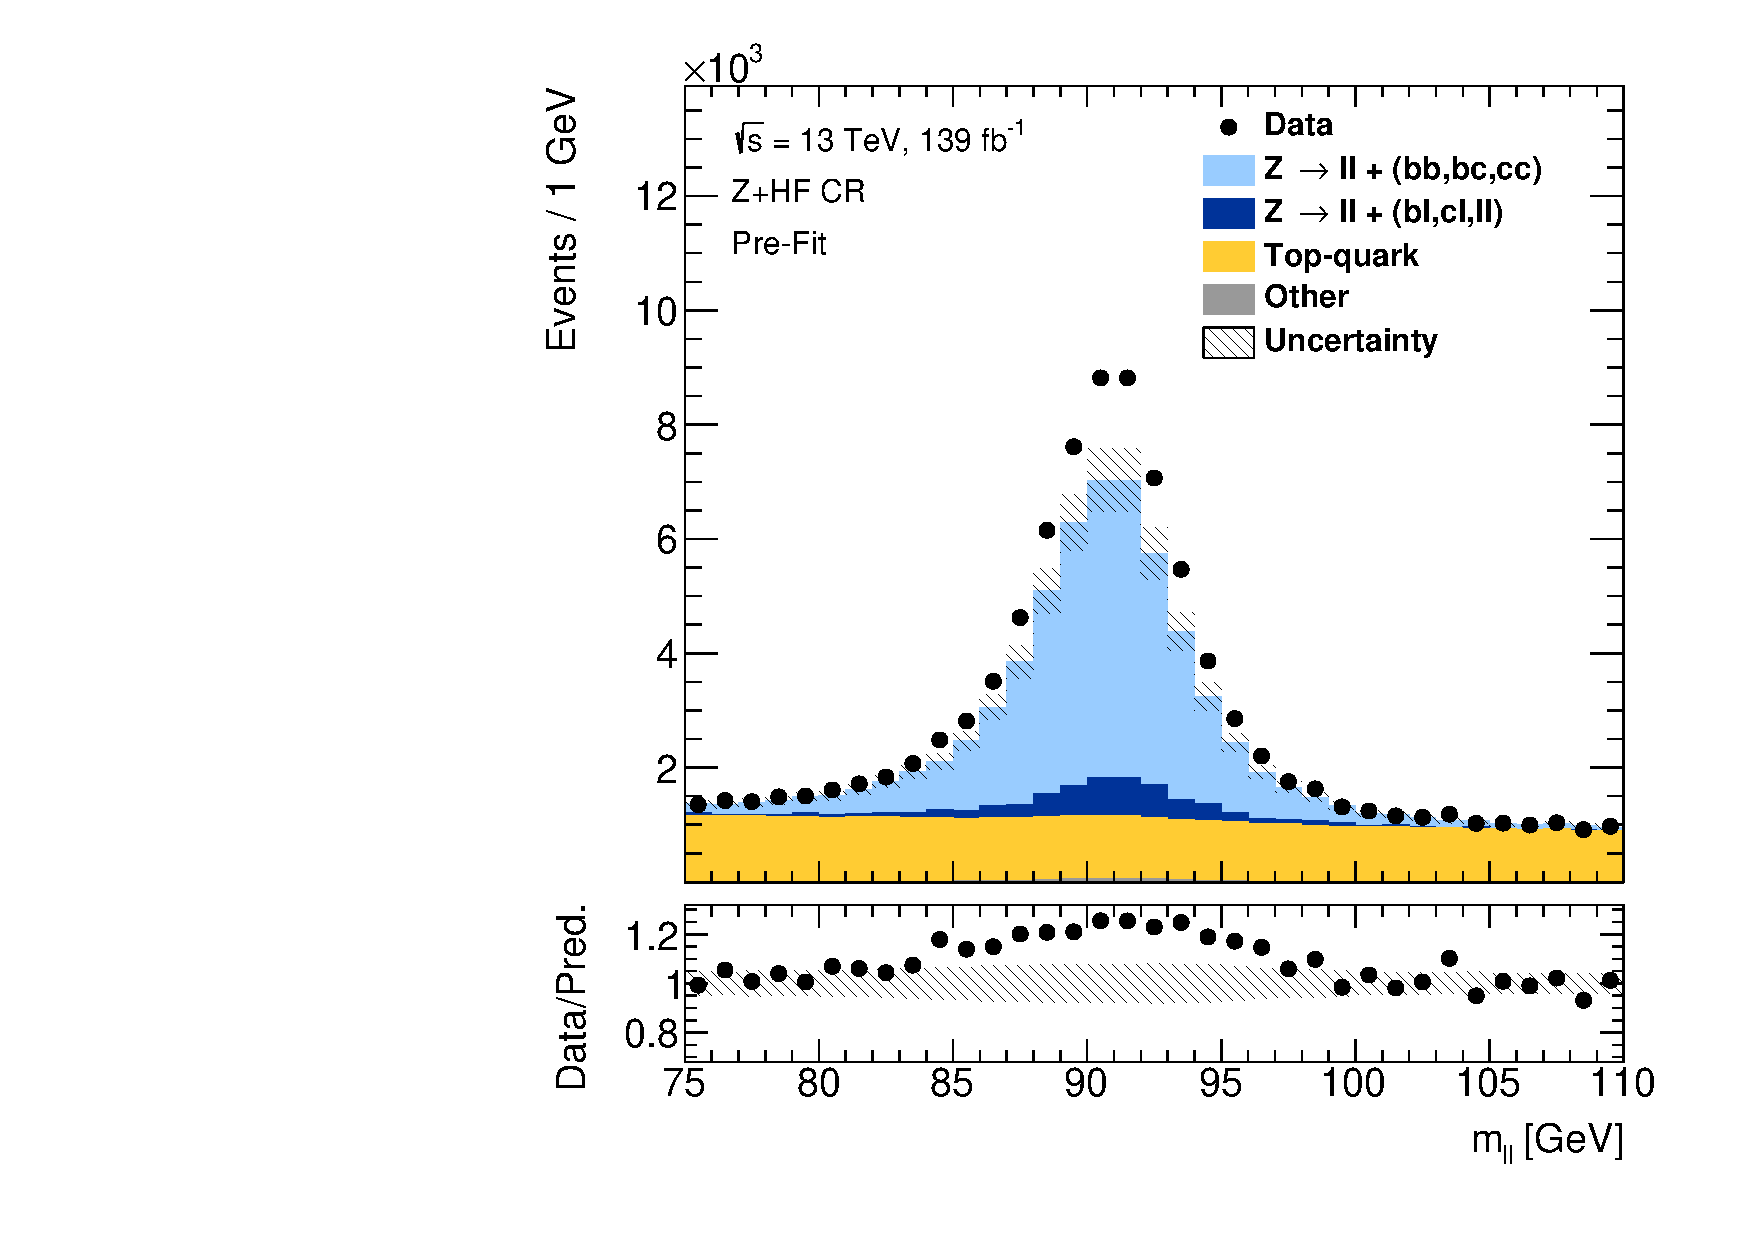
\includegraphics[width=0.65\textwidth]{zhfcr/Region_BMin0_incJet1_Y2015_DZllbbCR_T2_L2_distmLL_J2_Prefit_fixed}

    \column{0.5\textwidth}
    \centering

    \textbf{Post-fit}

    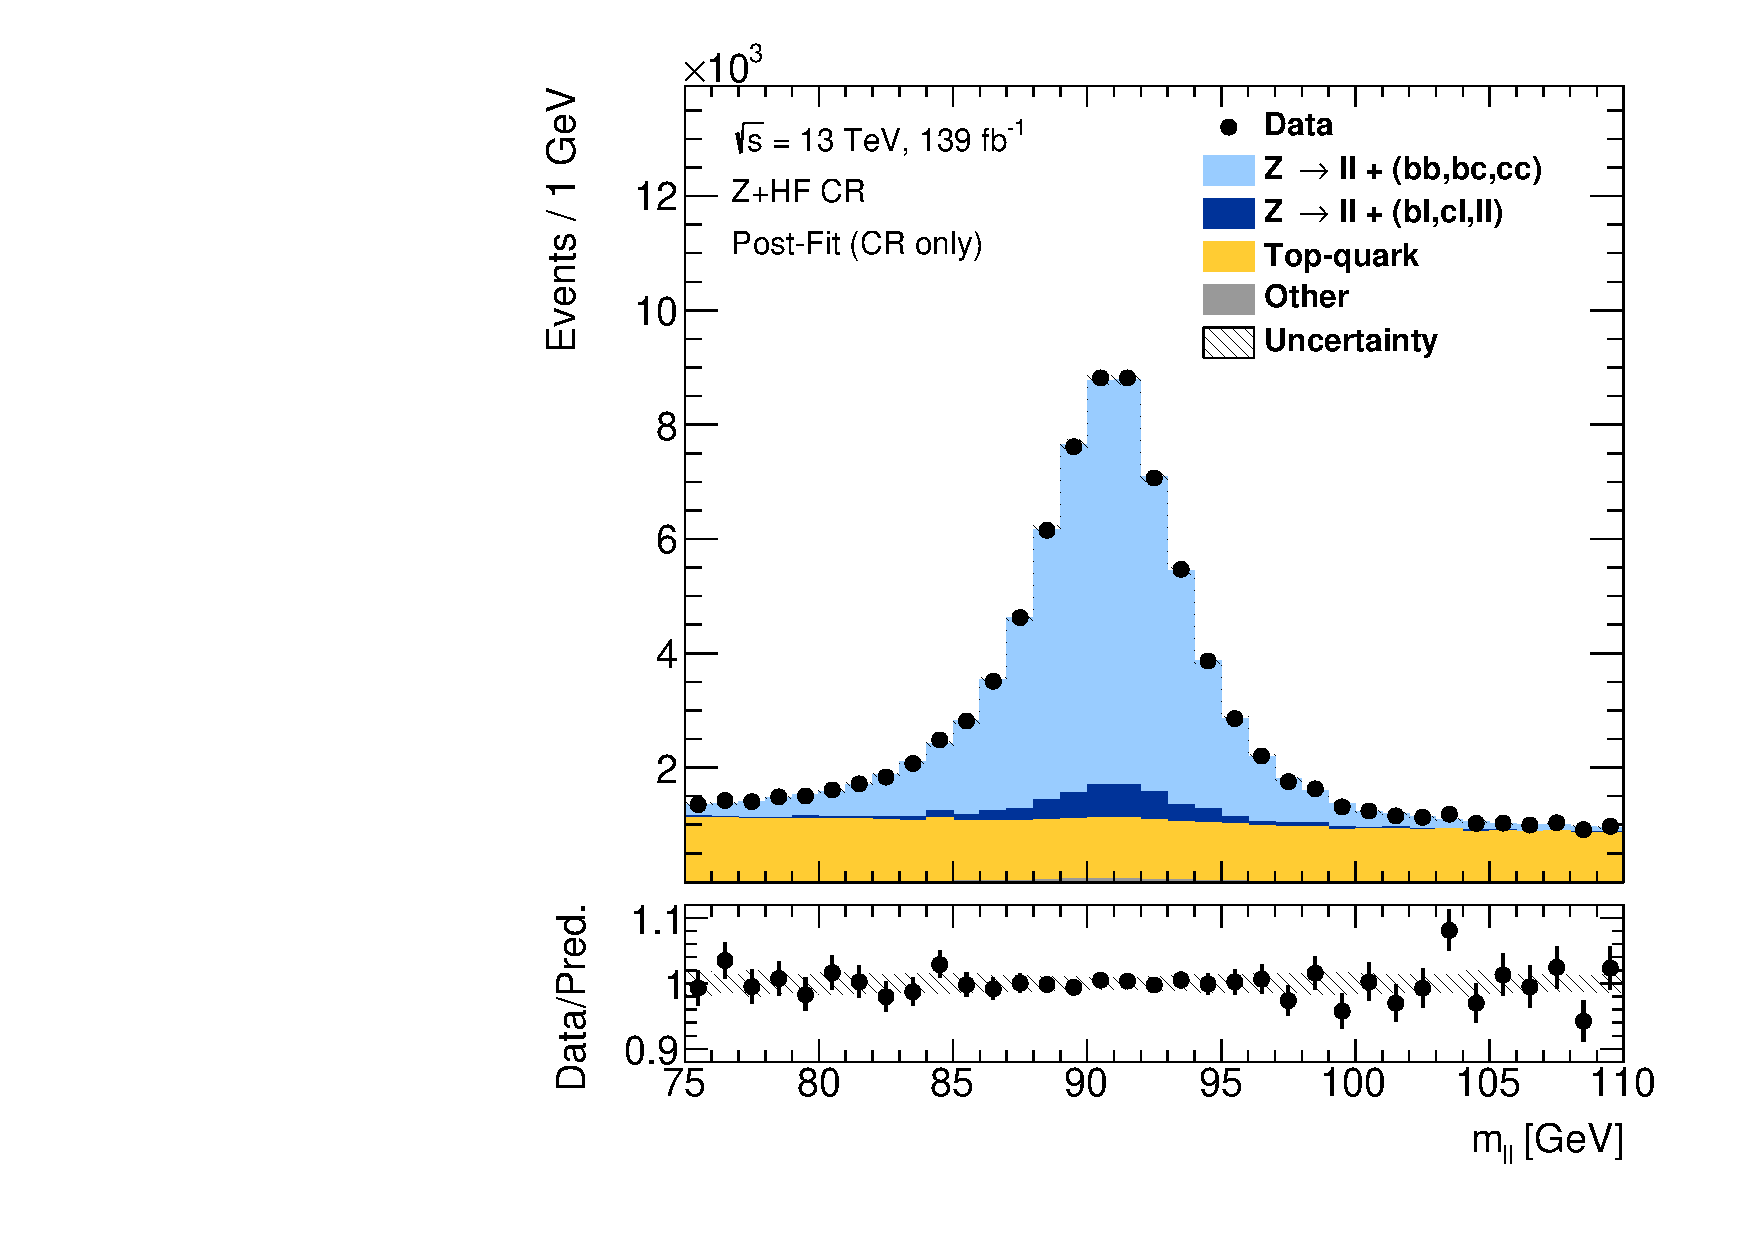
\includegraphics[width=0.65\textwidth]{zhfcr/Region_BMin0_incJet1_Y2015_DZllbbCR_T2_L2_distmLL_J2_GlobalFit_conditionnal_mu0_fixed}
  \end{columns}
\end{frame}

% ------------------------------------------------------------------------------

\begin{frame}{Background Estimation: ttbarfakes}
  Possibly add second slide
\end{frame}

% ------------------------------------------------------------------------------

\begin{frame}{Background Estimation: multi-jet}
  \centering

  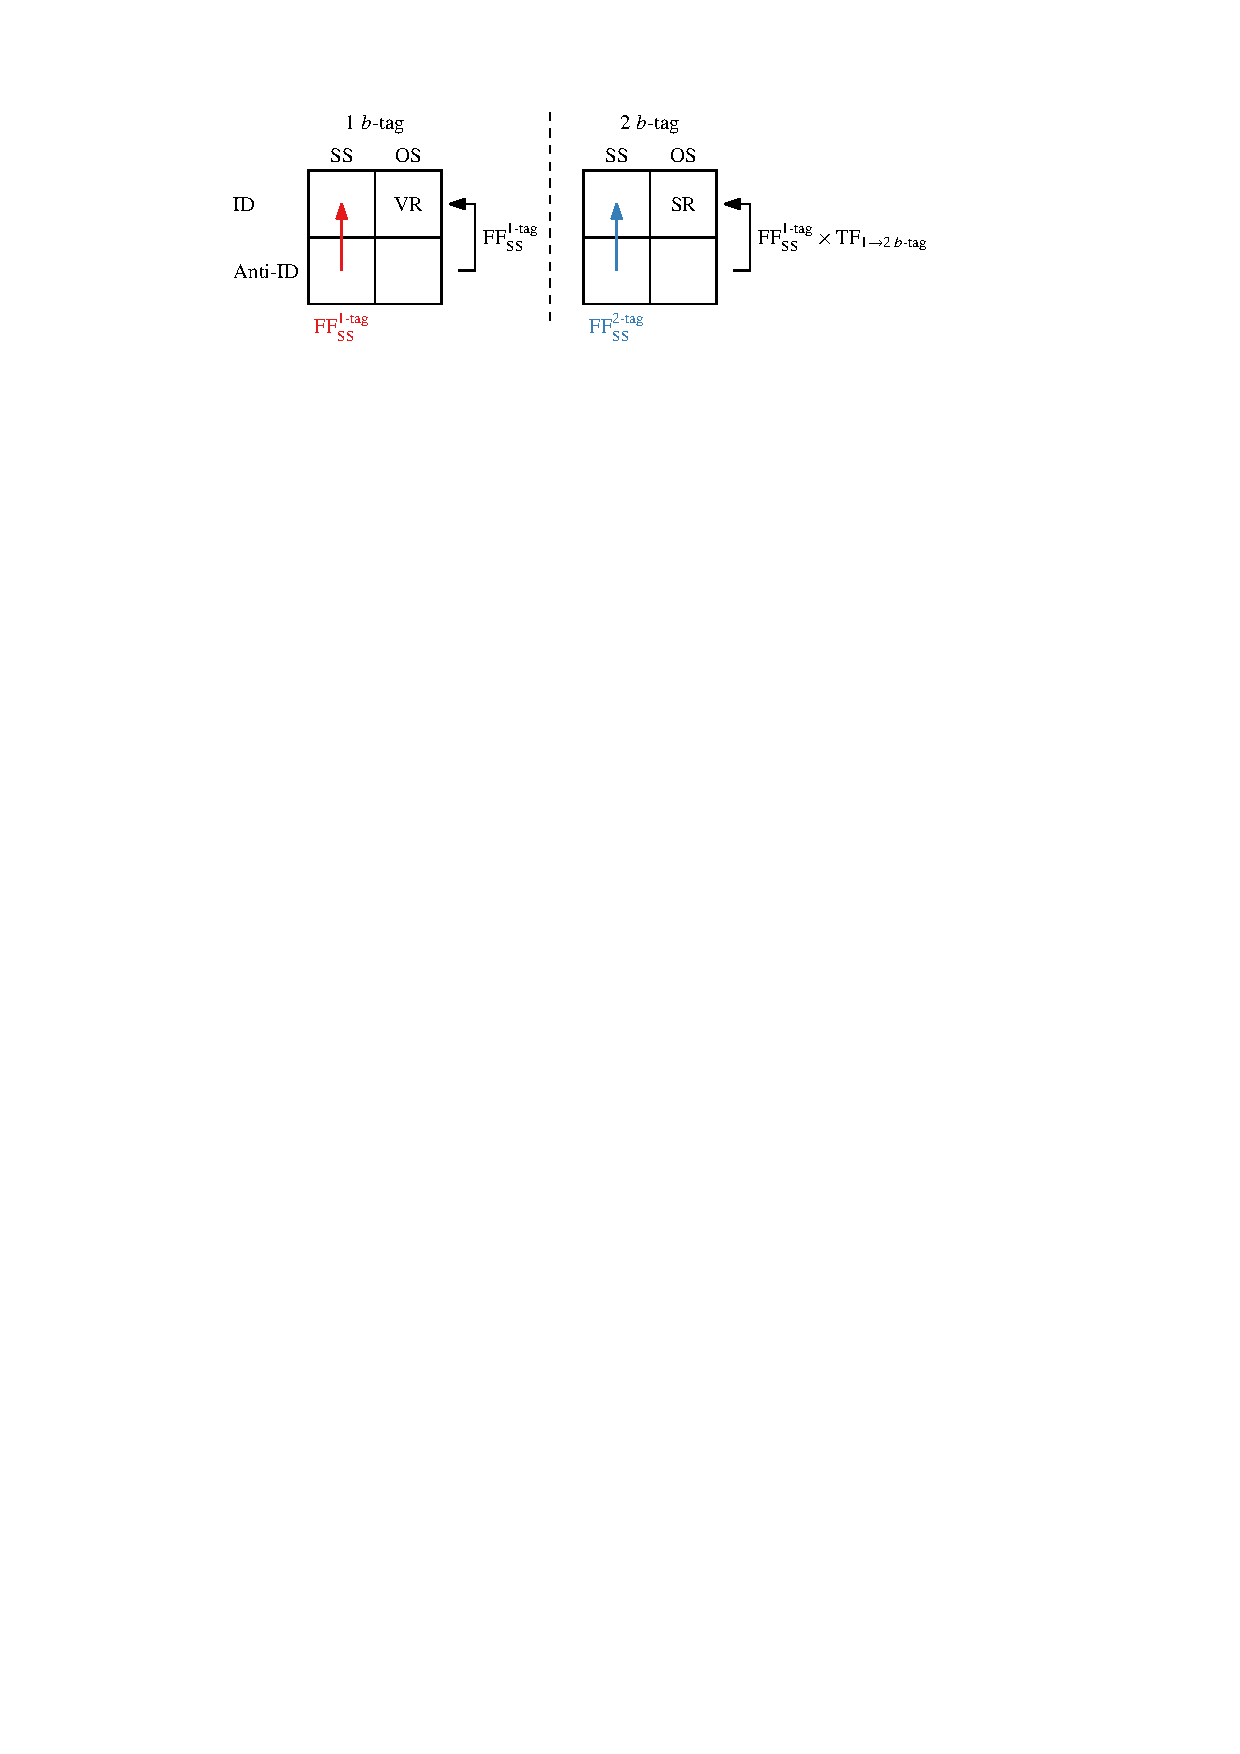
\includegraphics[width=0.6\textwidth]{fakefactors/regions}
\end{frame}

% ------------------------------------------------------------------------------

\begin{frame}{Multivariate Analysis}
  \begin{center}
    \footnotesize
    \begin{tabular}{lS[table-format=4.2(3)]S[table-format=5.1(3)]S[table-format=4.2(3)]}
      \toprule
      & \multicolumn{3}{c}{Channel}\\
      \cmidrule{2-4}
      & {\hadhad} & {\lephad SLT} & {\lephad LTT}\\
      \midrule
      SM~$HH$ ($gg$F+VBF) & 5.16 +- 0.84 & 5.9 +- 1.0   & 1.42 +- 0.24 \\
      Total Background    & 8414 +- 90   & 98430 +- 390 & 6357 +- 79 \\
      \midrule
      $S / B$ & {$6 \times 10^{-4}$} & {$6 \times 10^{-5}$} & {$2 \times 10^{-4}$} \\
      $S / \sqrt{B}$ & {$0.06$} & {$0.02$} & {$0.02$} \\
      \bottomrule
    \end{tabular}
  \end{center}

  \begin{itemize}
  \item Terrible significance
  \item Exploit kinematic properties of events to select signals / reject
    backgrounds
  \end{itemize}
\end{frame}

% ------------------------------------------------------------------------------

\begin{frame}{Discriminants}

  \begin{columns}[onlytextwidth]
    \column{0.5\textwidth}
    \centering

    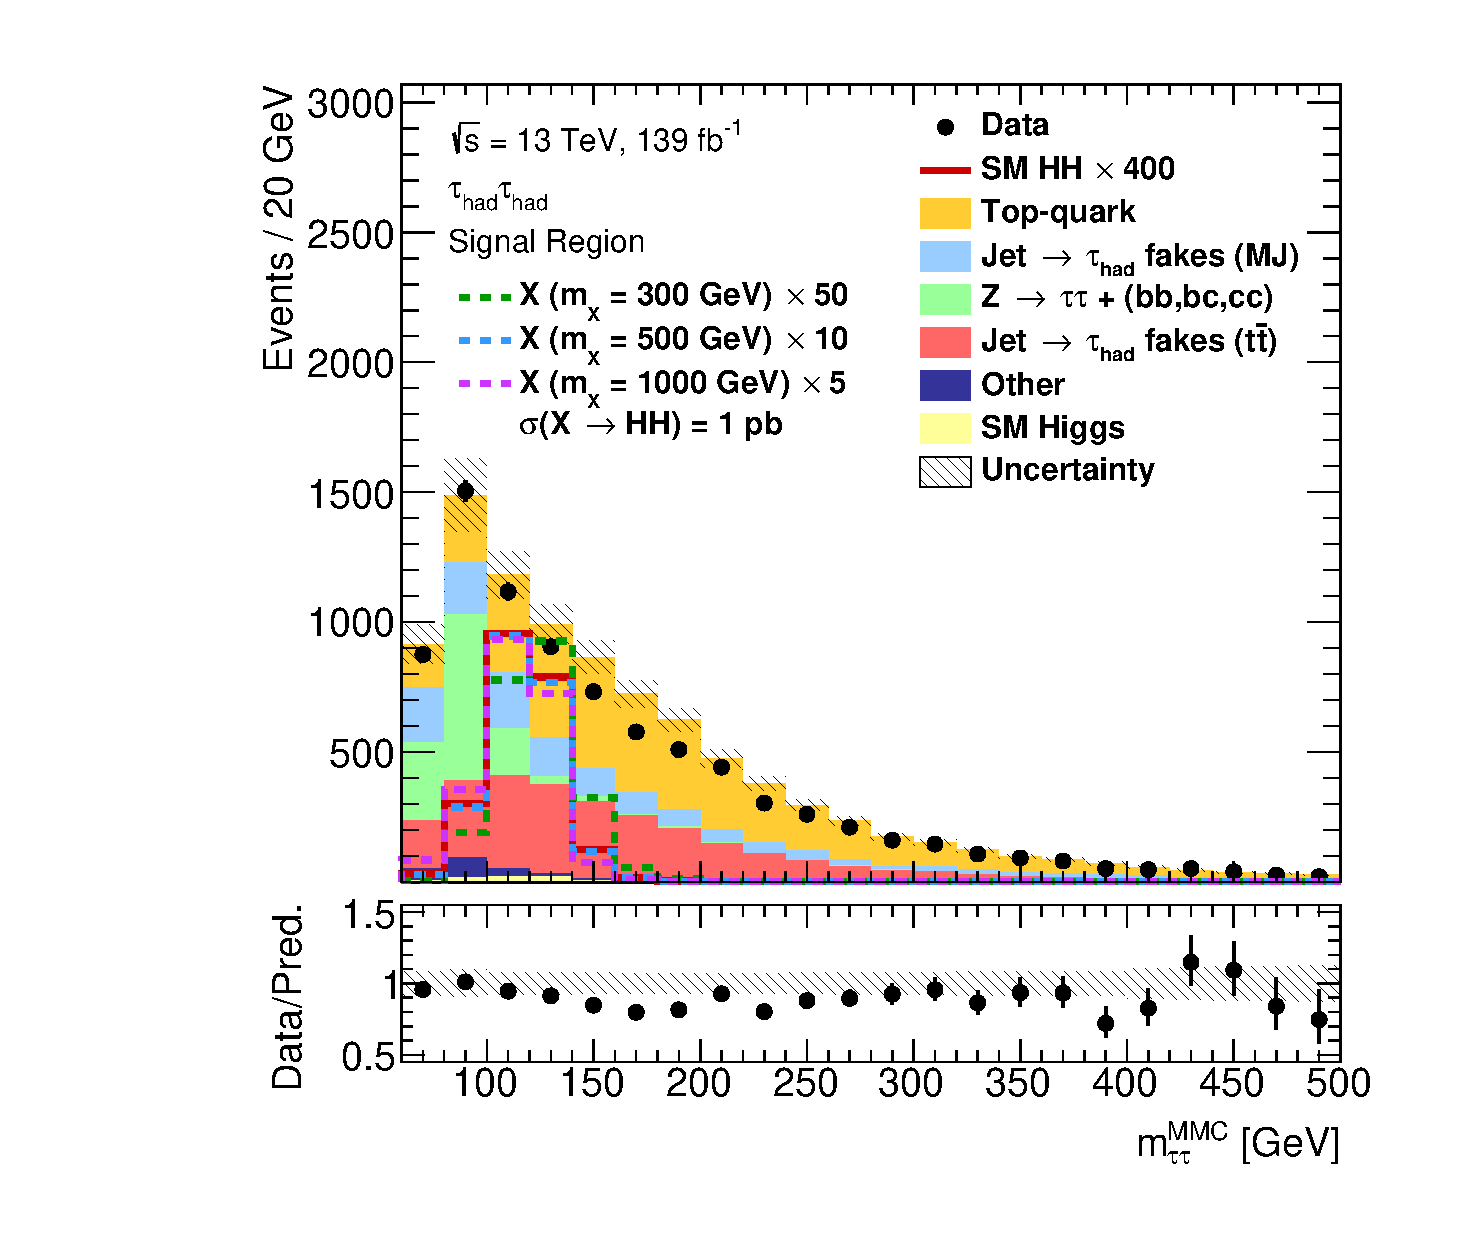
\includegraphics[width=0.8\textwidth]{mva/prefit/Region_BMin0_incJet1_distmMMC_J2_Y2015_DLLOS_T2_SpcTauHH_L0_Prefit}

    \column{0.5\textwidth}
    \centering

    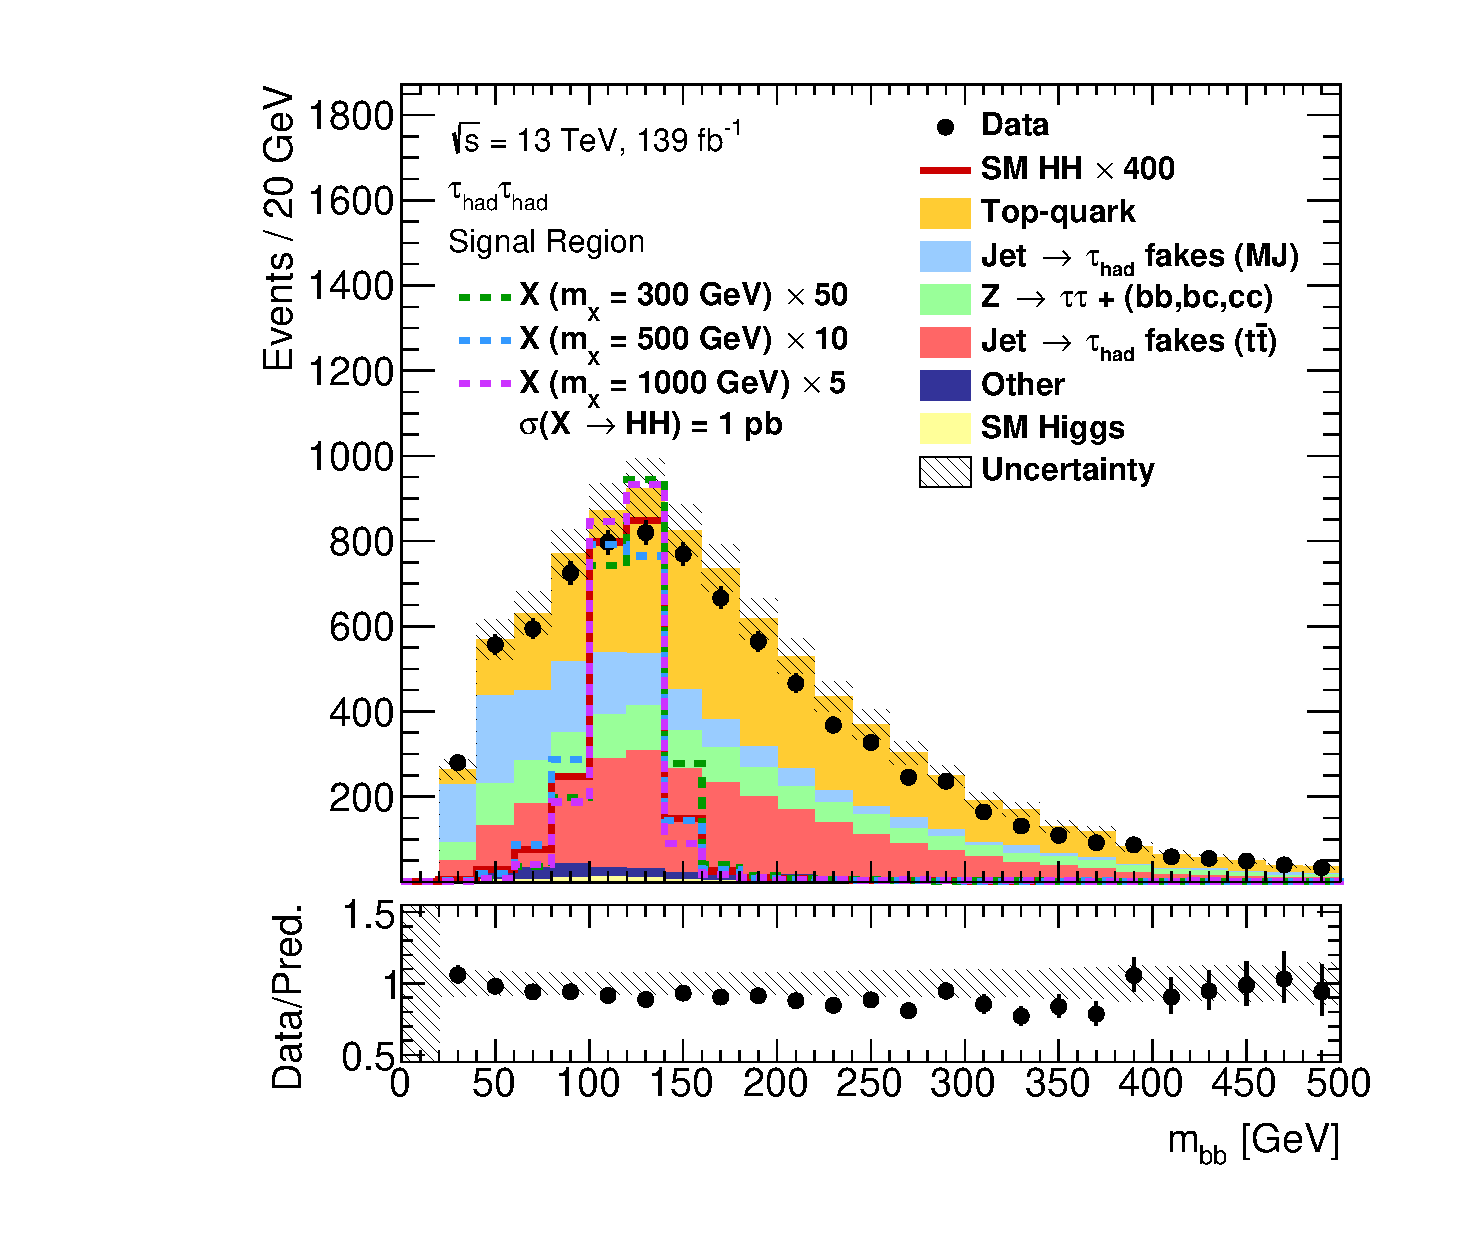
\includegraphics[width=0.8\textwidth]{mva/prefit/Region_BMin0_incJet1_distmBB_J2_Y2015_DLLOS_T2_SpcTauHH_L0_Prefit}
  \end{columns}

  % Two most important variables for SM HH

  \begin{itemize}
  \item \mMMC, \mBB, \mHH, $\Delta R(\tau, \tau)$, $\Delta R(b, b)$
  \end{itemize}
  
\end{frame}

% ------------------------------------------------------------------------------

\begin{frame}{Signal Extraction: non-resonant}
  \begin{columns}
    \column{0.5\textwidth}

    % BDT

    % NN is used in lephad

    \column{0.5\textwidth}
    \centering
    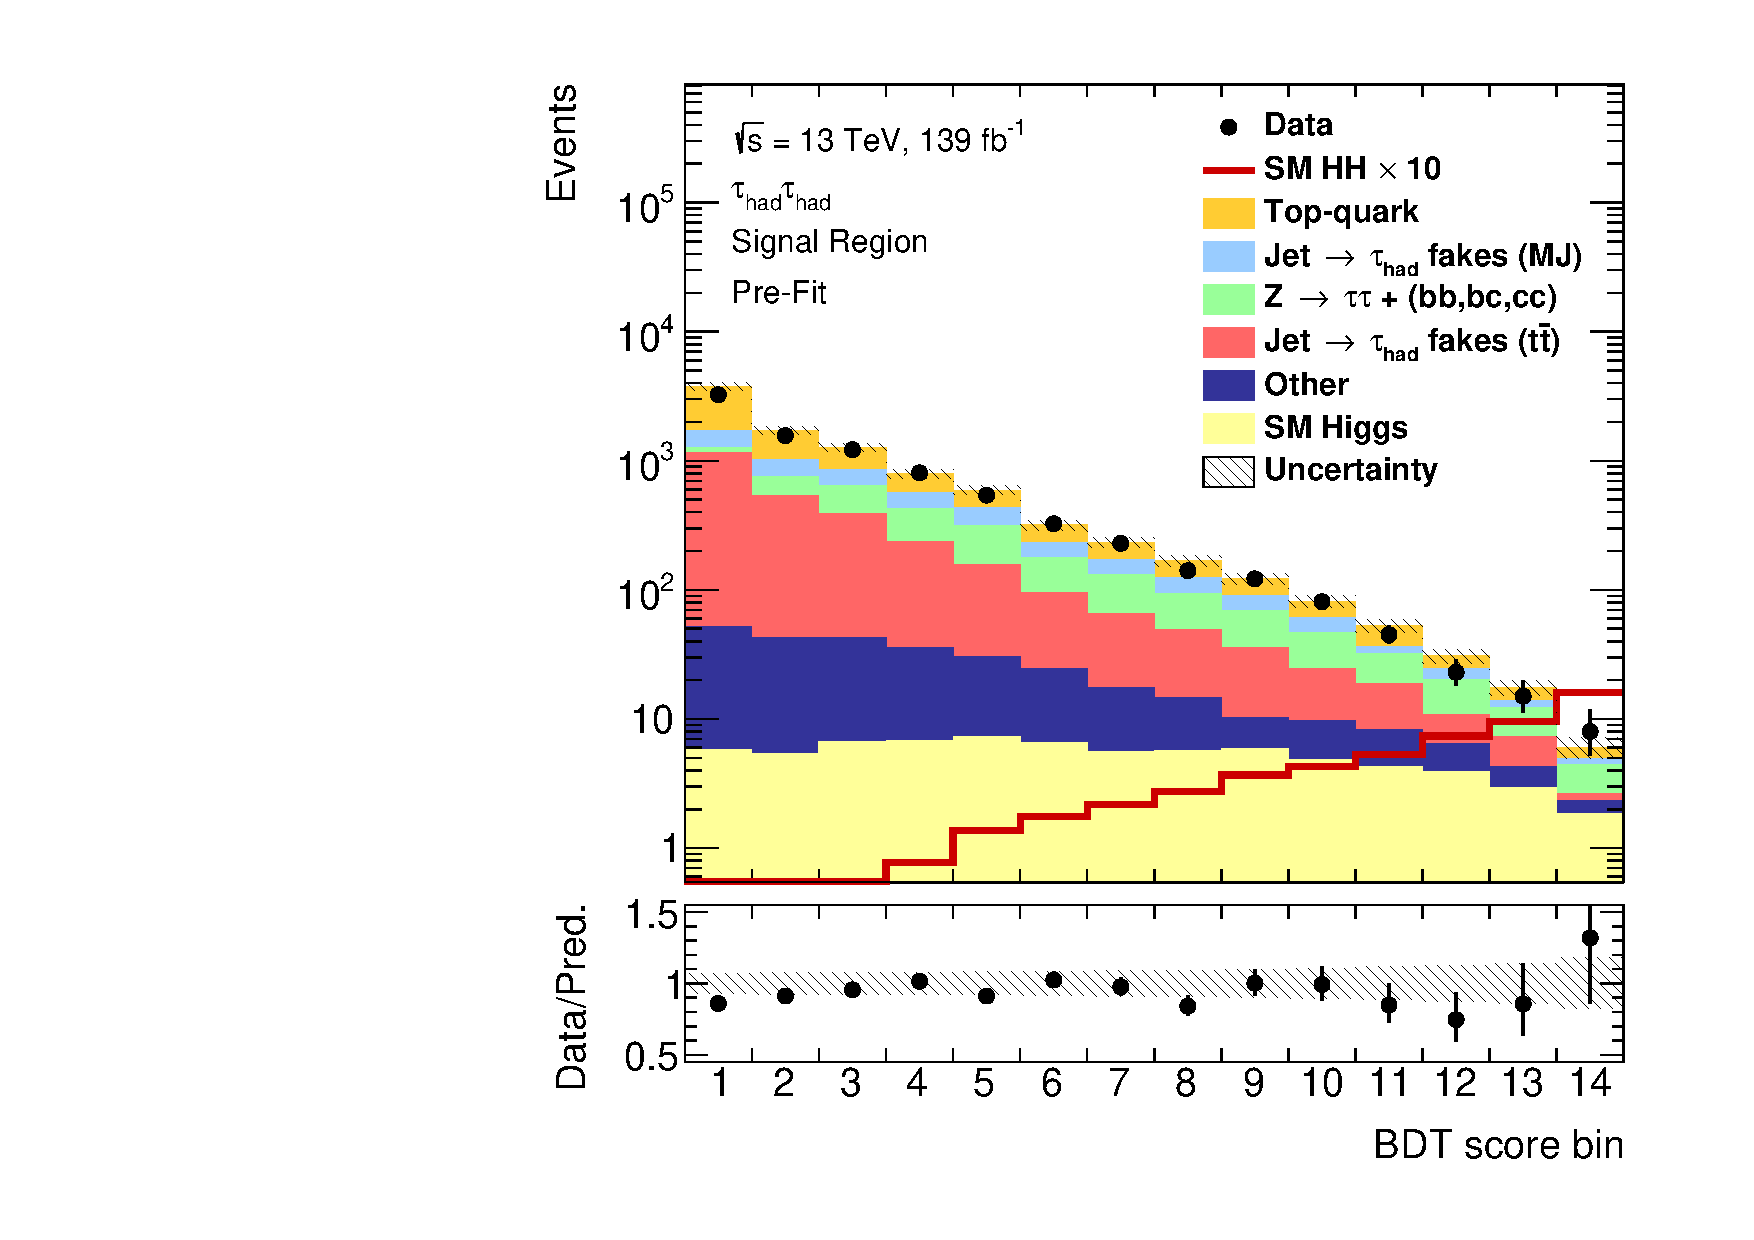
\includegraphics[width=0.8\textwidth]{mva/prefit/Region_BMin0_incJet1_distSMBDT_J2_Y2015_DLLOS_T2_SpcTauHH_L0_Prefitlog}
  \end{columns}
\end{frame}

% ------------------------------------------------------------------------------

\begin{frame}{Signal Extraction: resonant}
  \begin{columns}
    \column{0.5\textwidth}

    Classification task changes with $m_{X}$ \ra PNN

    \column{0.5\textwidth}
    \centering

    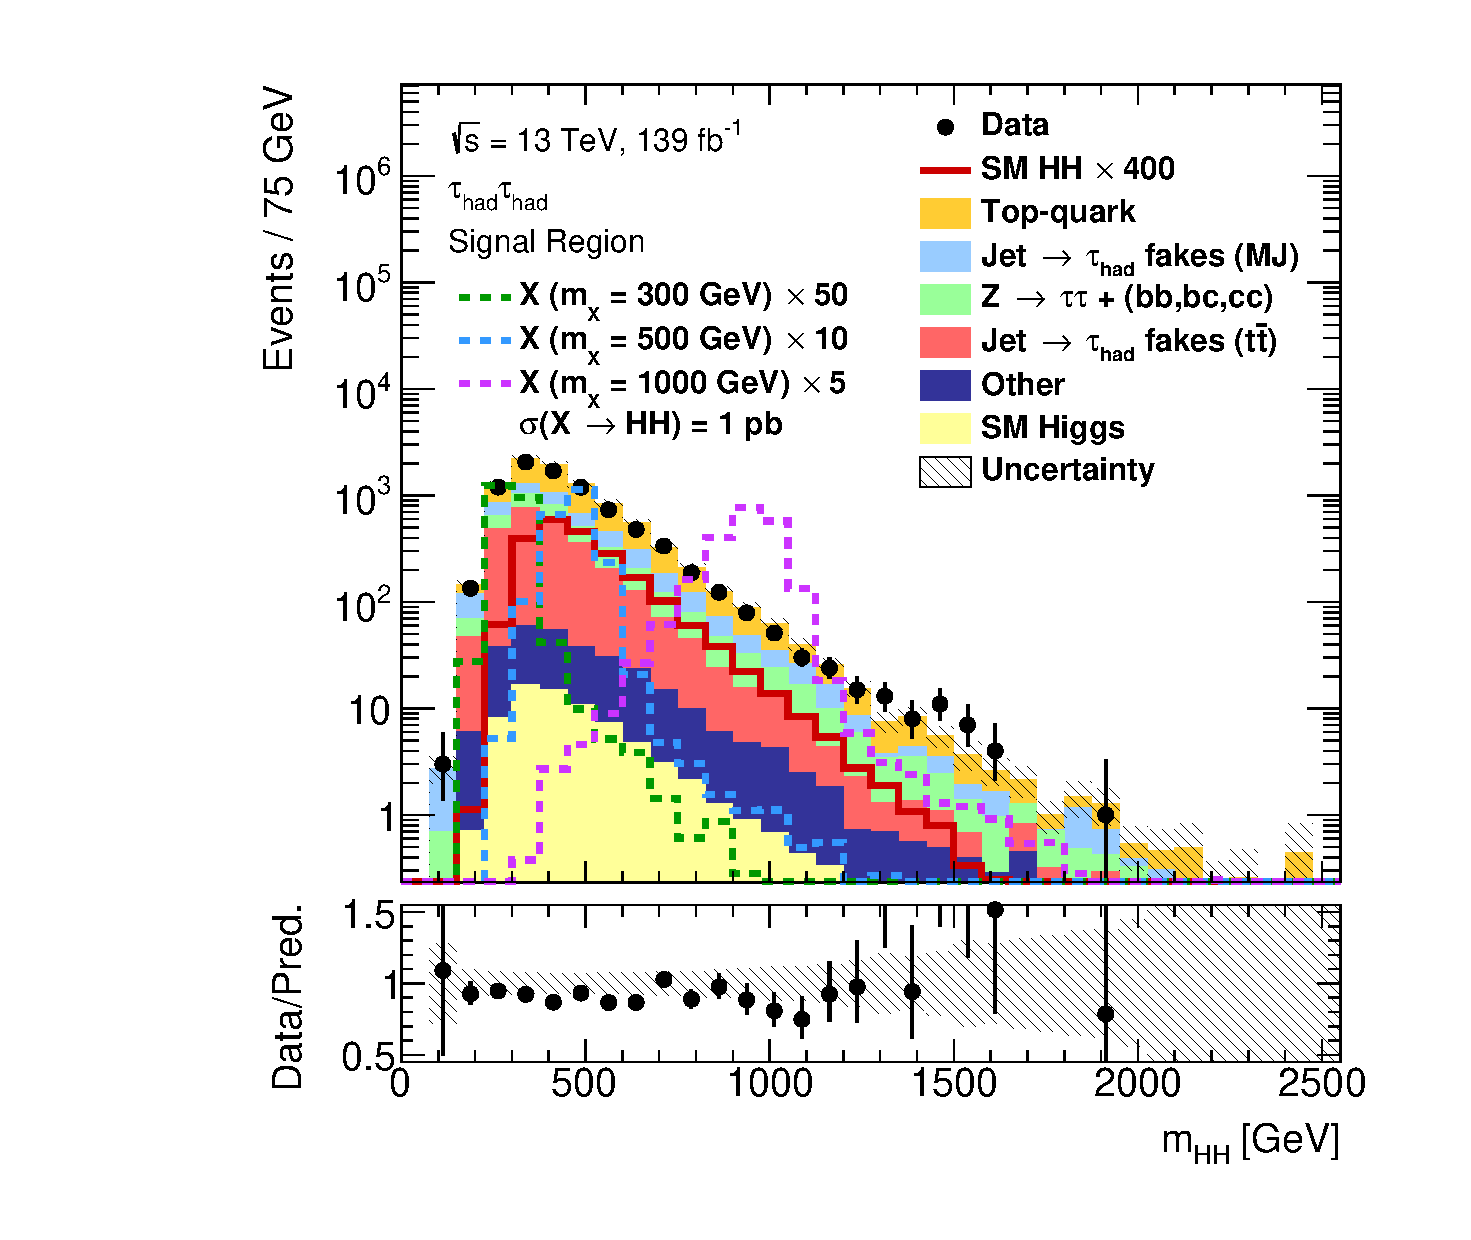
\includegraphics[width=0.8\textwidth]{mva/prefit/Region_BMin0_incJet1_distmHH_J2_Y2015_DLLOS_T2_SpcTauHH_L0_Prefit_logy}
  \end{columns}


\end{frame}

% ------------------------------------------------------------------------------

\begin{frame}{Statistical Analysis I}
\end{frame}

% ------------------------------------------------------------------------------

\begin{frame}{Uncertainties}
  \begin{columns}[onlytextwidth]
    \column{0.4\textwidth}

    Table of uncertainties

    Largely limited by the number of observed events

    Largest uncertainties are:
    - Background statistical precision
    - Single Higgs boson bkg modelling
    - Top quark bkg.\ modelling

    \column{0.6\textwidth}
    \centering

    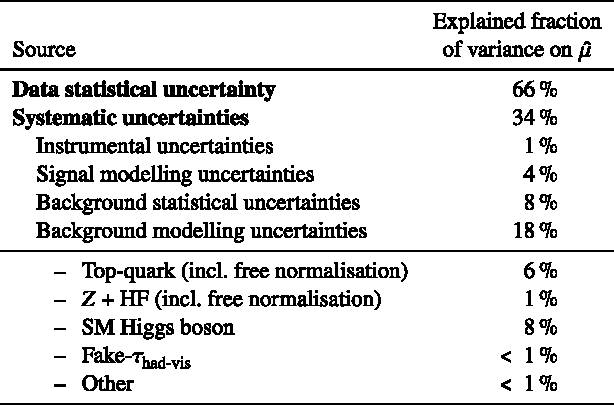
\includegraphics[width=0.9\textwidth]{uncertainty_table}
  \end{columns}


\end{frame}

% ------------------------------------------------------------------------------

\begin{frame}{Results}
  \begin{columns}[onlytextwidth]
    \column{0.5\textwidth}

    Highest expected sensitivity of any single channel
    \begin{itemize}
    \item CMS H $\mu < 3.3$ (obs.) $\mu < 5.2$ (exp.)
    \end{itemize}

    Largest expected sensitivity of any channel

    \column{0.5\textwidth}
    \centering

    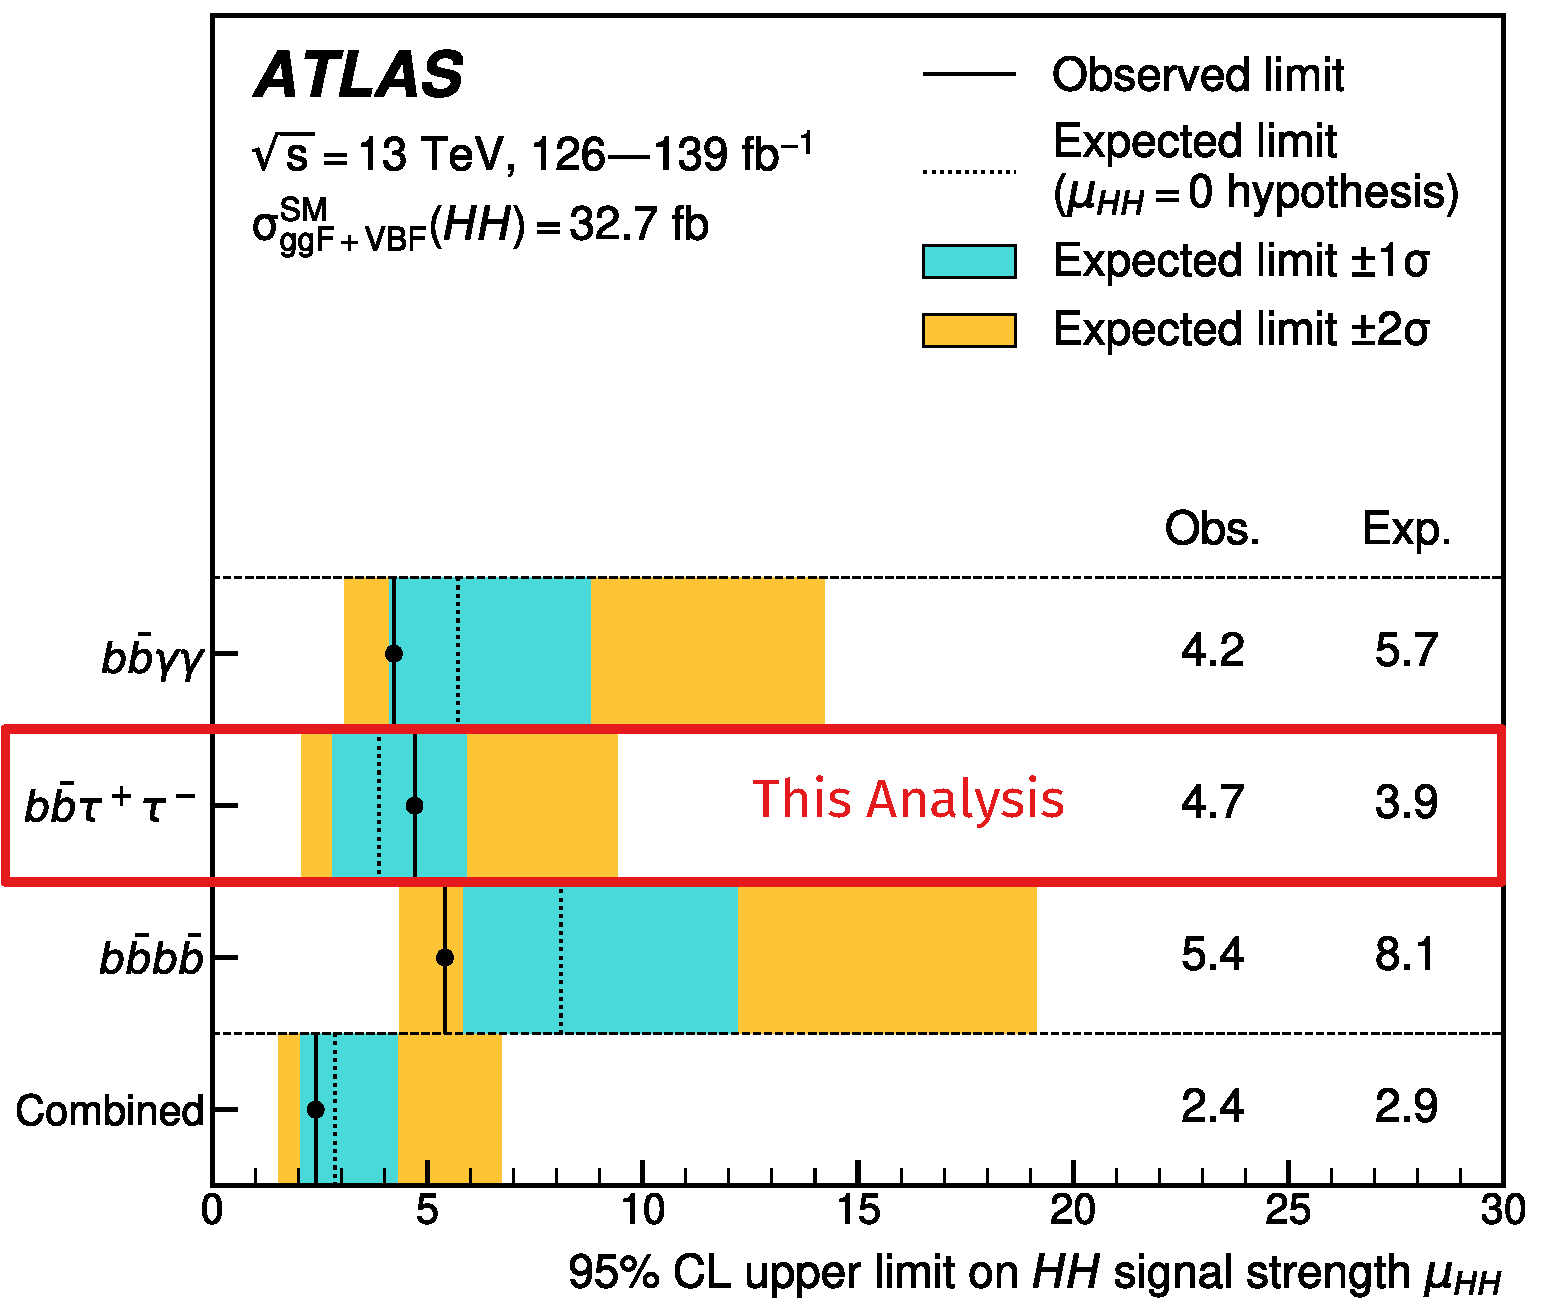
\includegraphics[width=0.9\textwidth]{discussion/results_139ifb}

  \end{columns}
\end{frame}

% ------------------------------------------------------------------------------

\begin{frame}{Results II}
  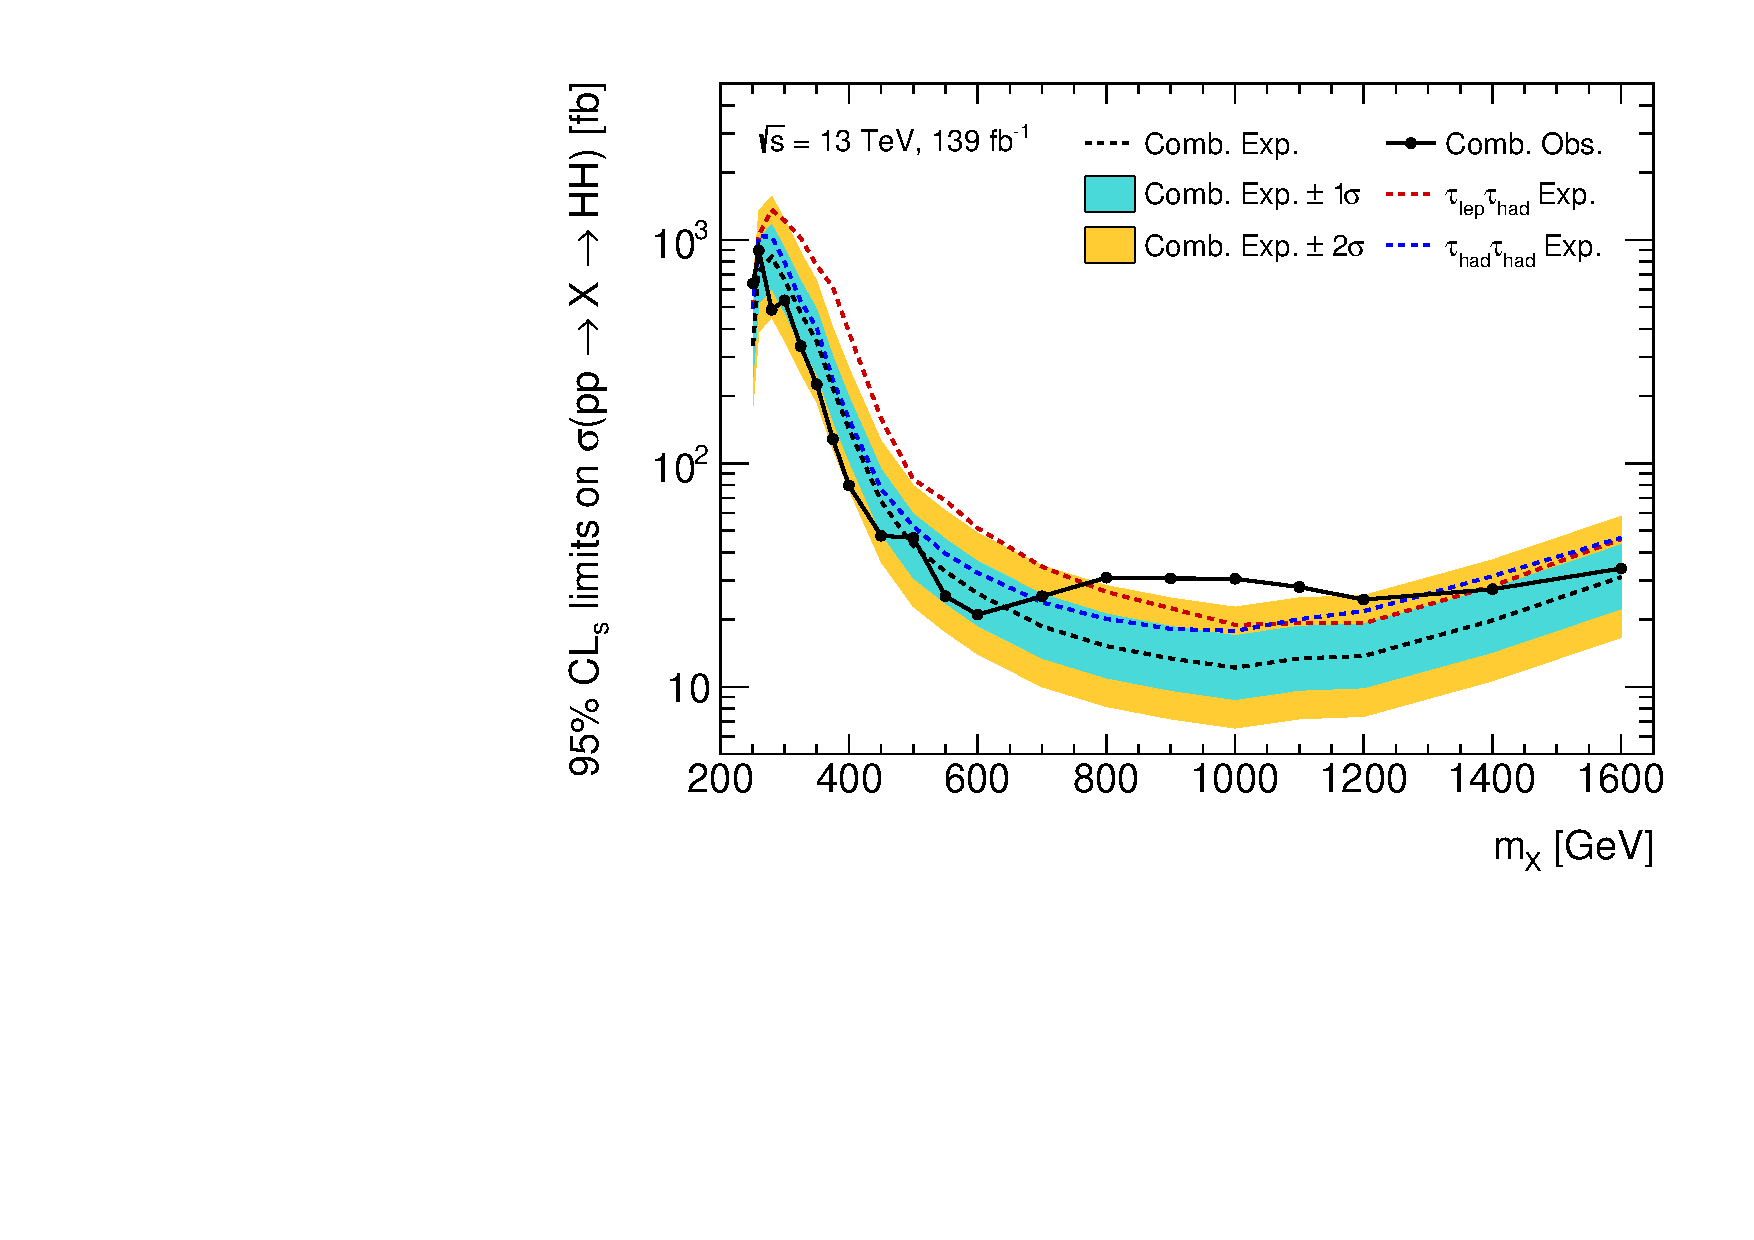
\includegraphics[width=0.5\textwidth]{results_res/resonant_upper_limits}
\end{frame}

% ------------------------------------------------------------------------------

\begin{frame}{Constraining the Higgs Boson Self-Coupling}

  \begin{center}
    \begin{overpic}[width=0.35\textwidth]{feynman_graphs/di_higgs_effective}
      \put(115,20){$\kappa_{\lambda} = \lambda_{HHH} / \lambda_{HHH}^{\text{SM}}$}
    \end{overpic}
  \end{center}

  What if new physics changes the Higgs Boson self-coupling?
  \begin{itemize}
  \item Heavy new particles might contribute (reduce to effective coupling)
  \item Reinterpret the SM~\HH search \ra limits on xsec vs.\ $\kappa_{\lambda}$
  \end{itemize}
\end{frame}

% ------------------------------------------------------------------------------

\begin{frame}{Phenomenology of Anomalous $\kappa_{\lambda}$}
  \begin{columns}
    \column{0.5\textwidth}
    \centering

    $HH$ production cross section

    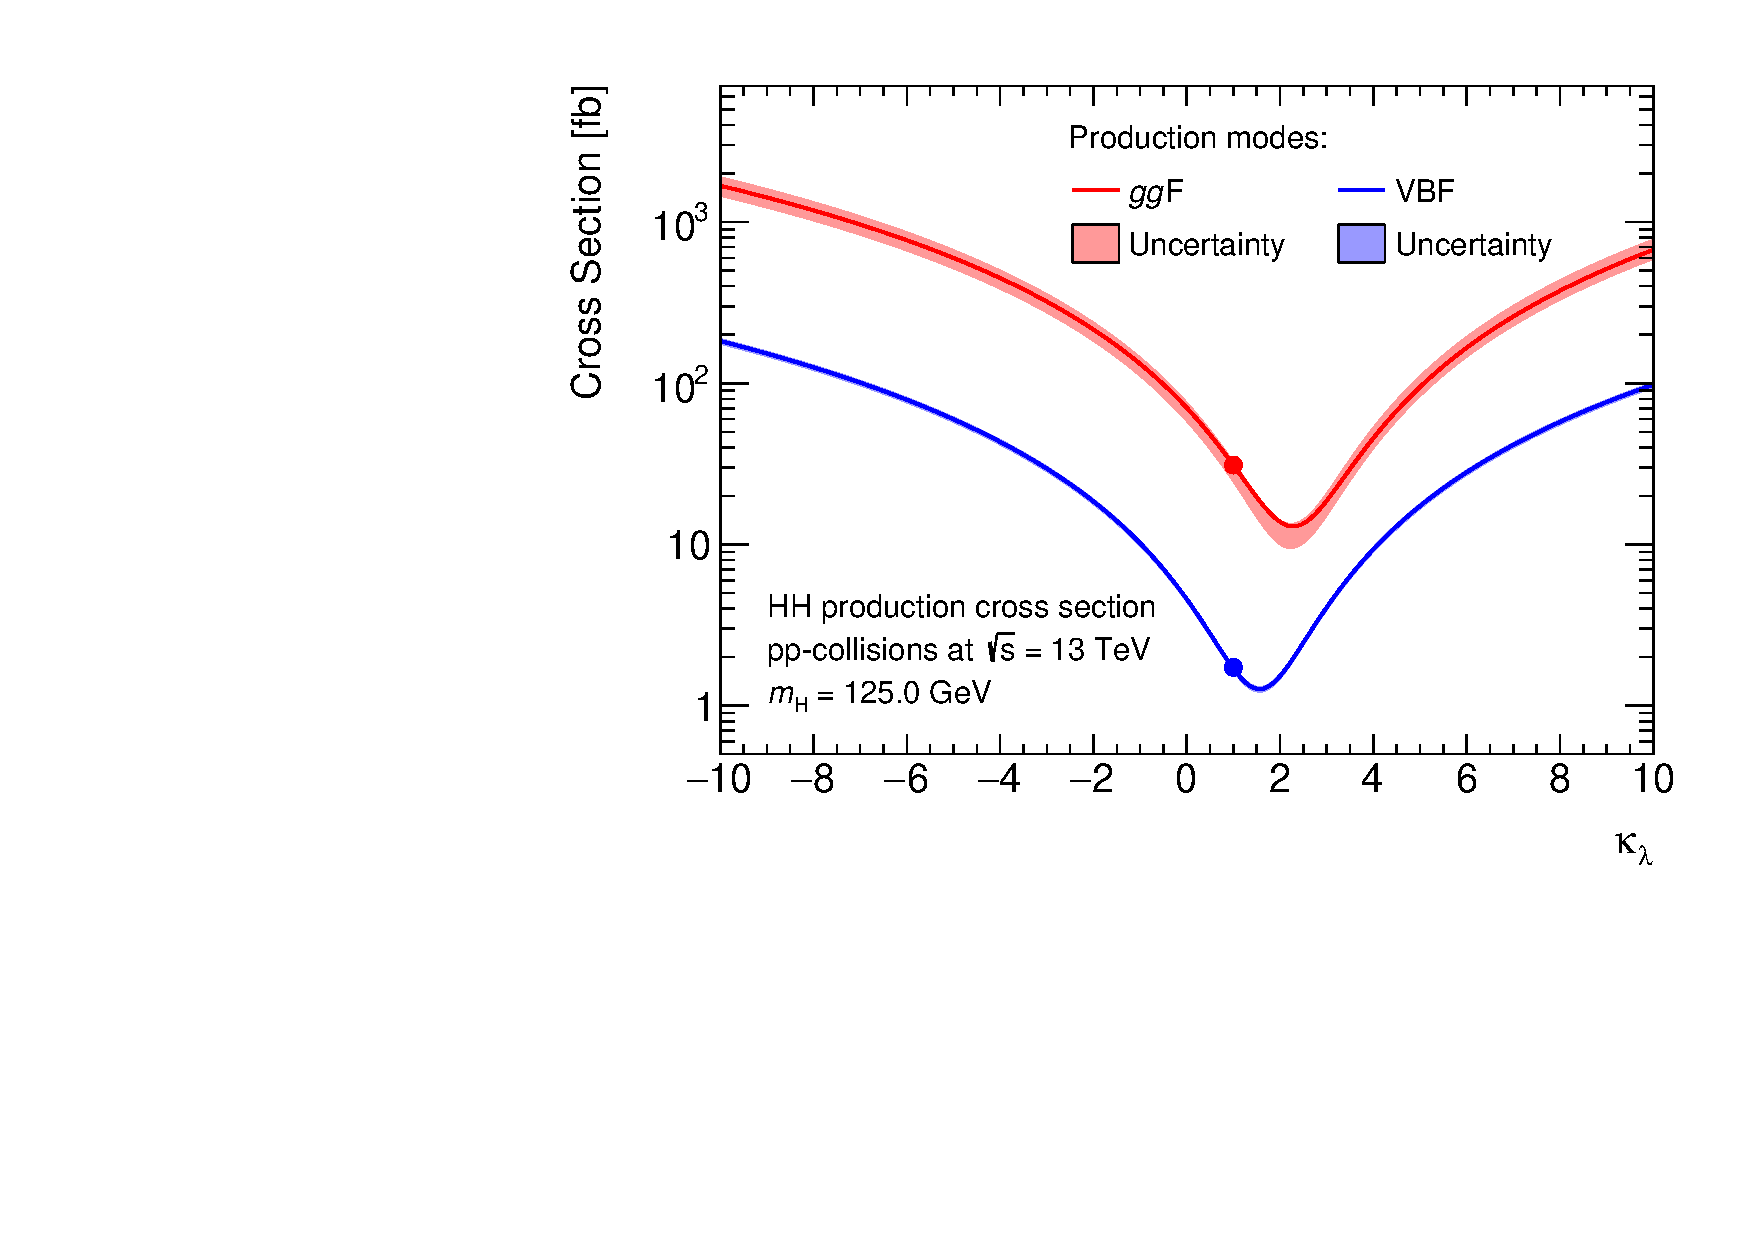
\includegraphics[width=0.9\textwidth]{self_coupling/hh_xsec}

    \column{0.5\textwidth}
    \centering

    \mHH-spectra

    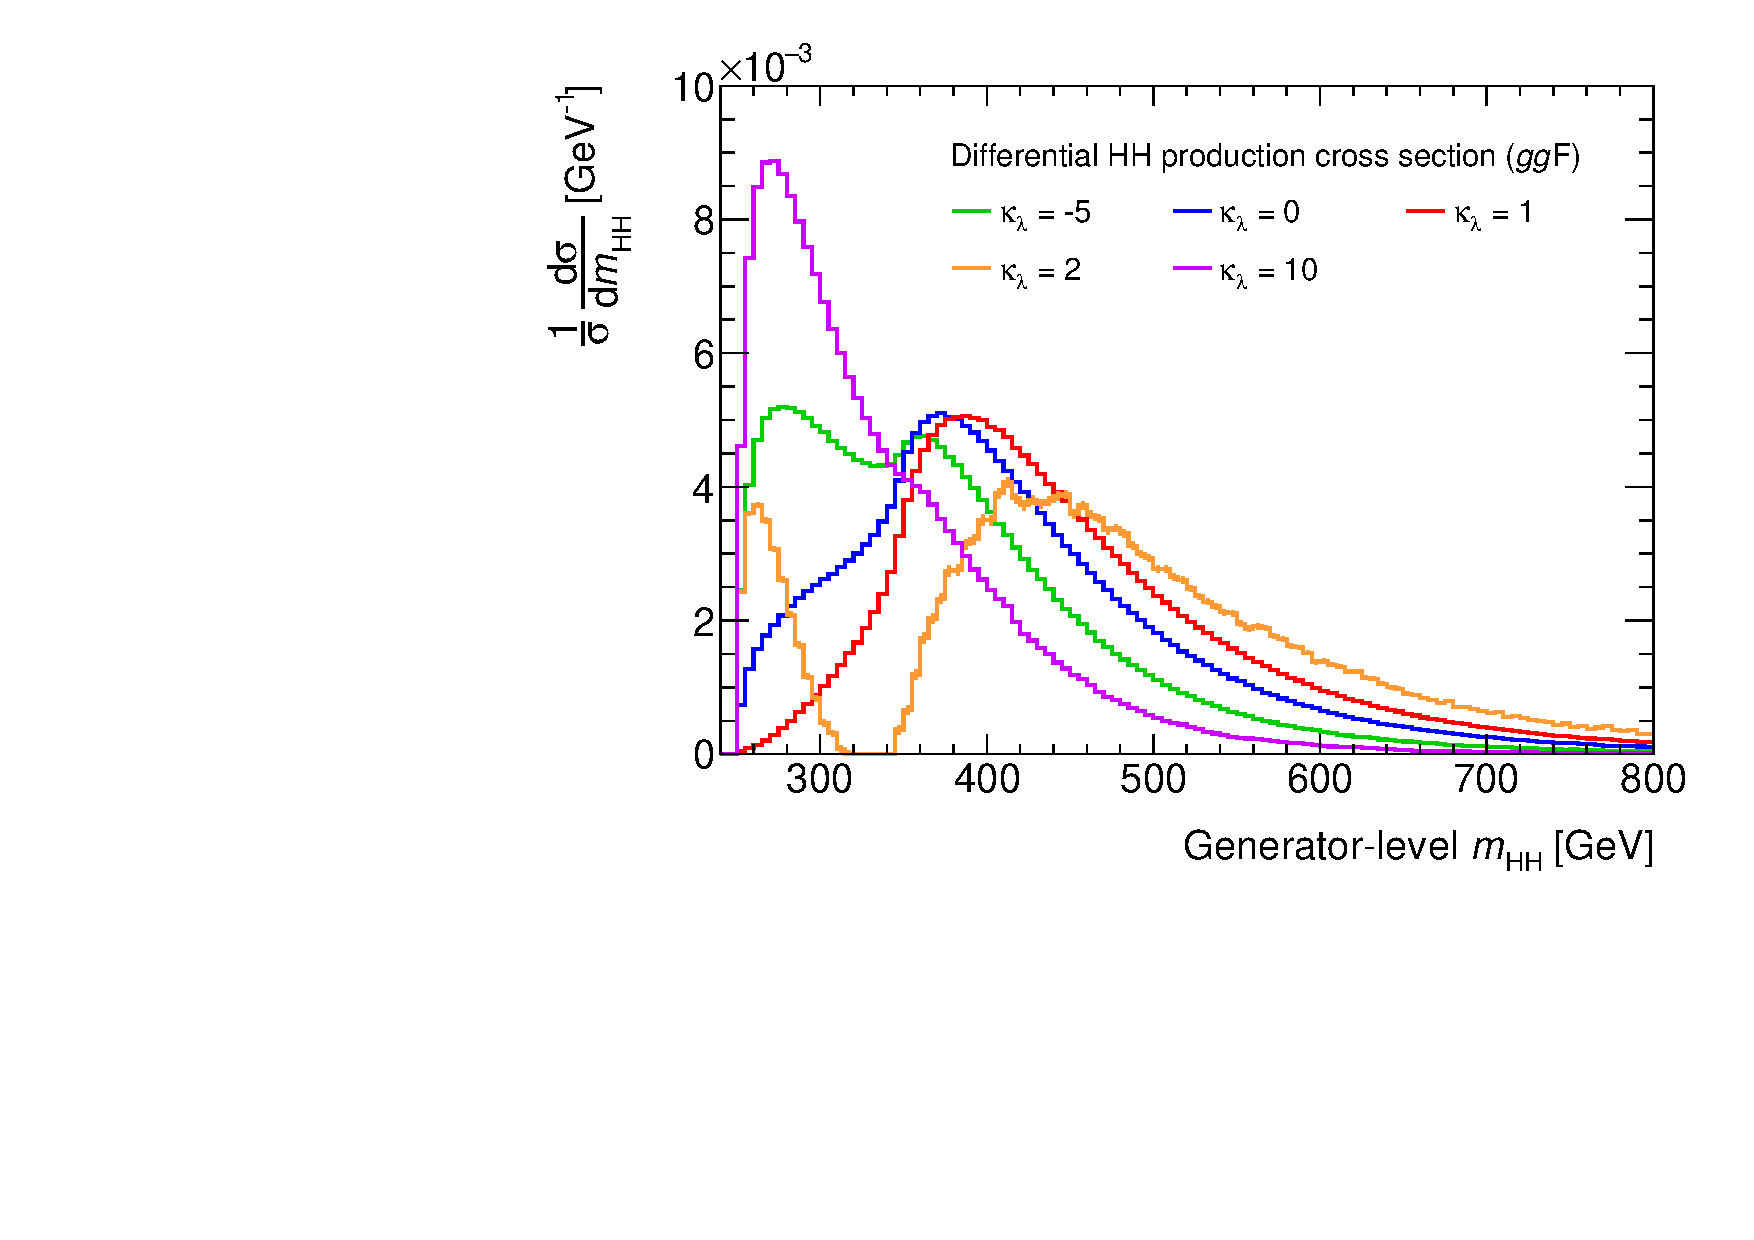
\includegraphics[width=0.9\textwidth]{self_coupling/hh_mhh_vs_klam}
  \end{columns}

  \begin{itemize}
  \item
  \end{itemize}
\end{frame}

% ------------------------------------------------------------------------------p

\begin{frame}{Constraining the Higgs Boson Self-Coupling}

  \begin{columns}[onlytextwidth]
    \column{0.5\textwidth}




    \textbf{Limitations:}
    \begin{itemize}
    \item Not accounting for changes in
    \end{itemize}

    \column{0.5\textwidth} \centering

    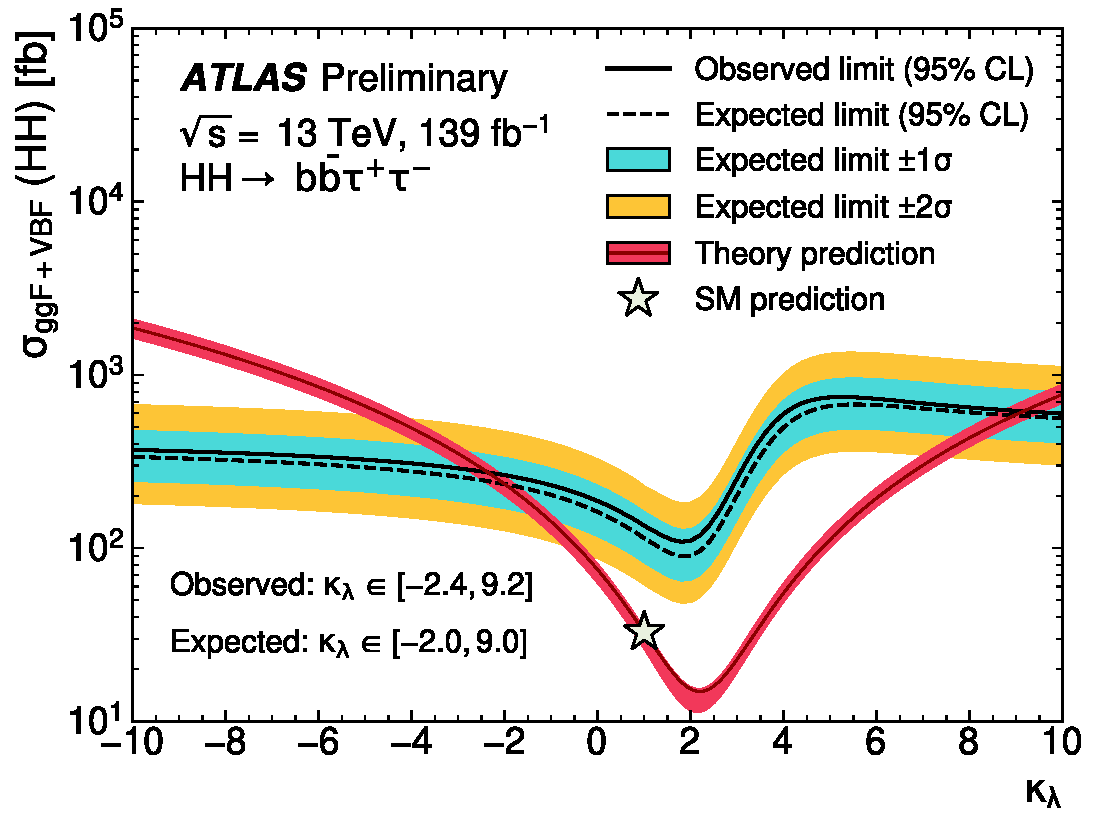
\includegraphics[width=0.95\textwidth]{self_coupling/klam_scan_result}
  \end{columns}




  % Limitations
  %
  % - Does not account for xsec / BR changes for single higgs
  %
  % - Not a statistically proper confidence interval
\end{frame}

% ------------------------------------------------------------------------------

\begin{frame}{Conclusion \& Outlook}
  Evidence expected at the HL-LHC (discovery would be realistic)
\end{frame}

% ------------------------------------------------------------------------------

{ % all template changes are local to this group.
  \setbeamertemplate{navigation symbols}{}
  \setbeamercolor{background canvas}{bg=black}
  \begin{frame}<article:0>[plain]
    \begin{tikzpicture}[remember picture,overlay]
      \node[at=(current page.center)] {
        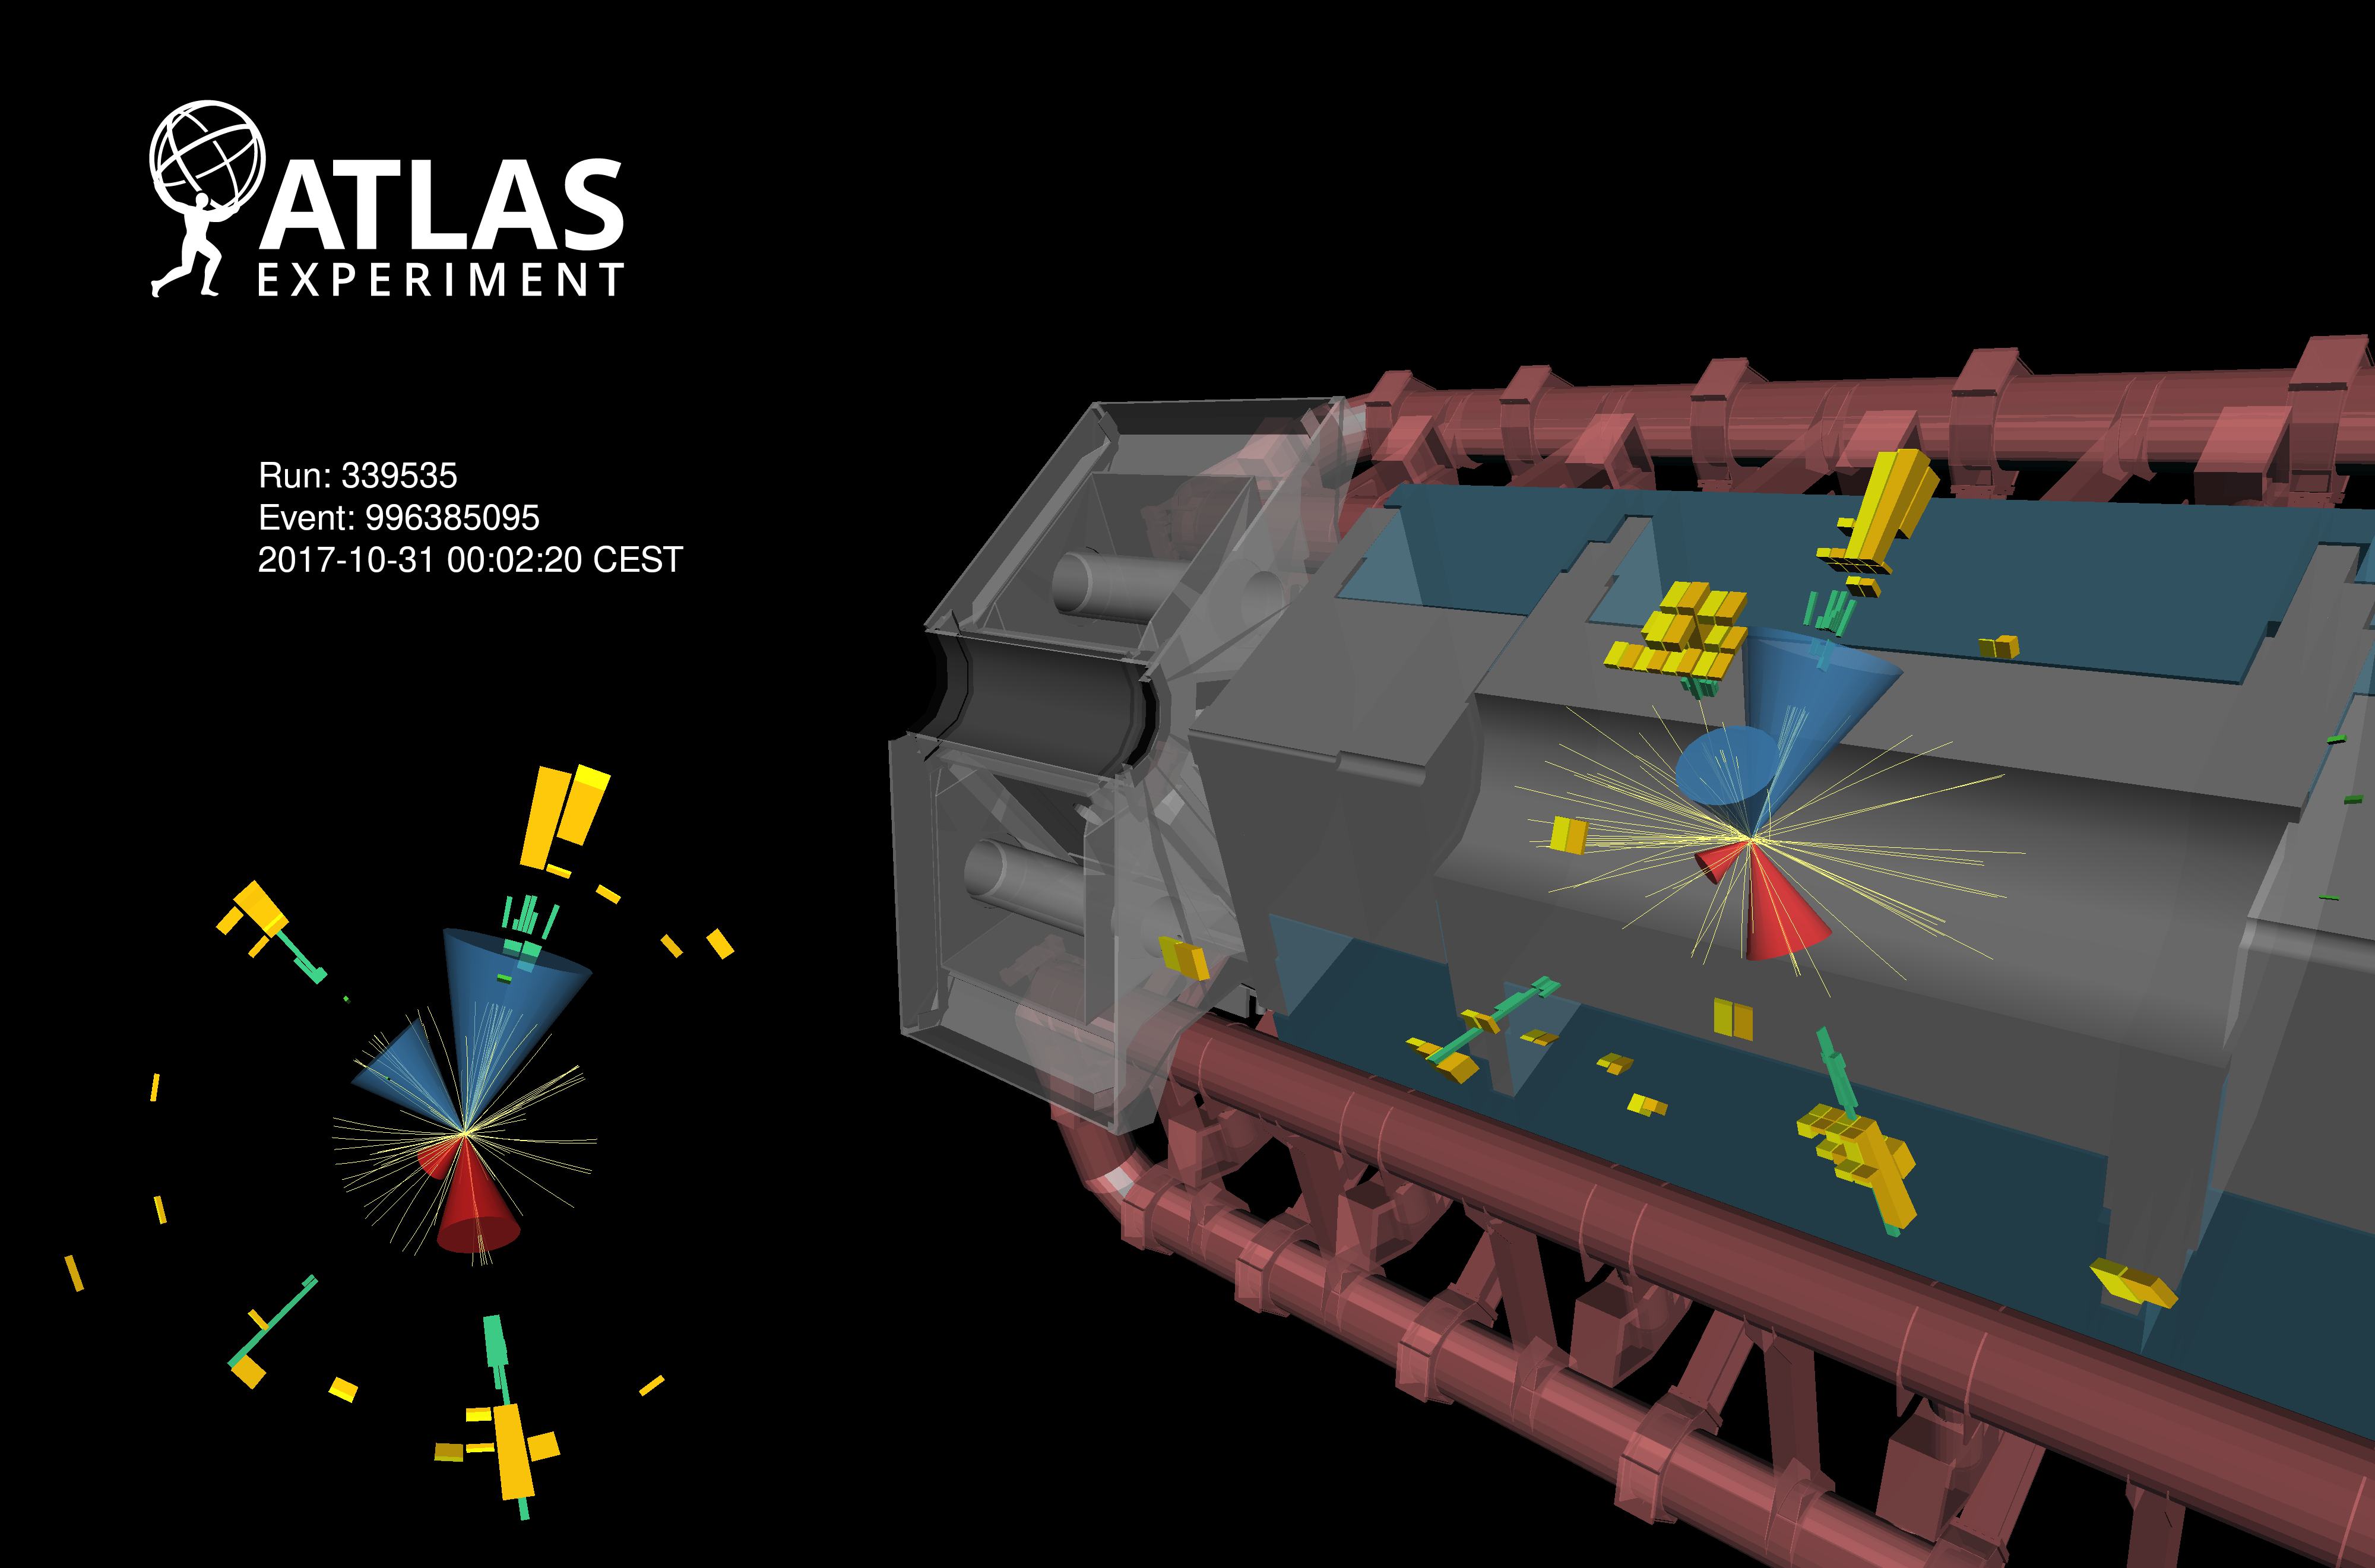
\includegraphics[keepaspectratio,
        width=\paperwidth,
        height=\paperheight]{event_displays/hadhad}
      };
      % \node at (0.73\paperwidth,0.46\paperheight) {
      %   \textcolor{White}{$HH \ra {\color{bjetblue}b\bar{b}}{\color{taured}\tau_\mu\tauhad}$ candidate event}
      % };
    \end{tikzpicture}
  \end{frame}
}

% ------------------------------------------------------------------------------

{ % all template changes are local to this group.
  \setbeamercolor{background canvas}{bg=black}
  \begin{frame}[plain]
    \begin{tikzpicture}[remember picture,overlay]
      \node[at=(current page.center)] {
        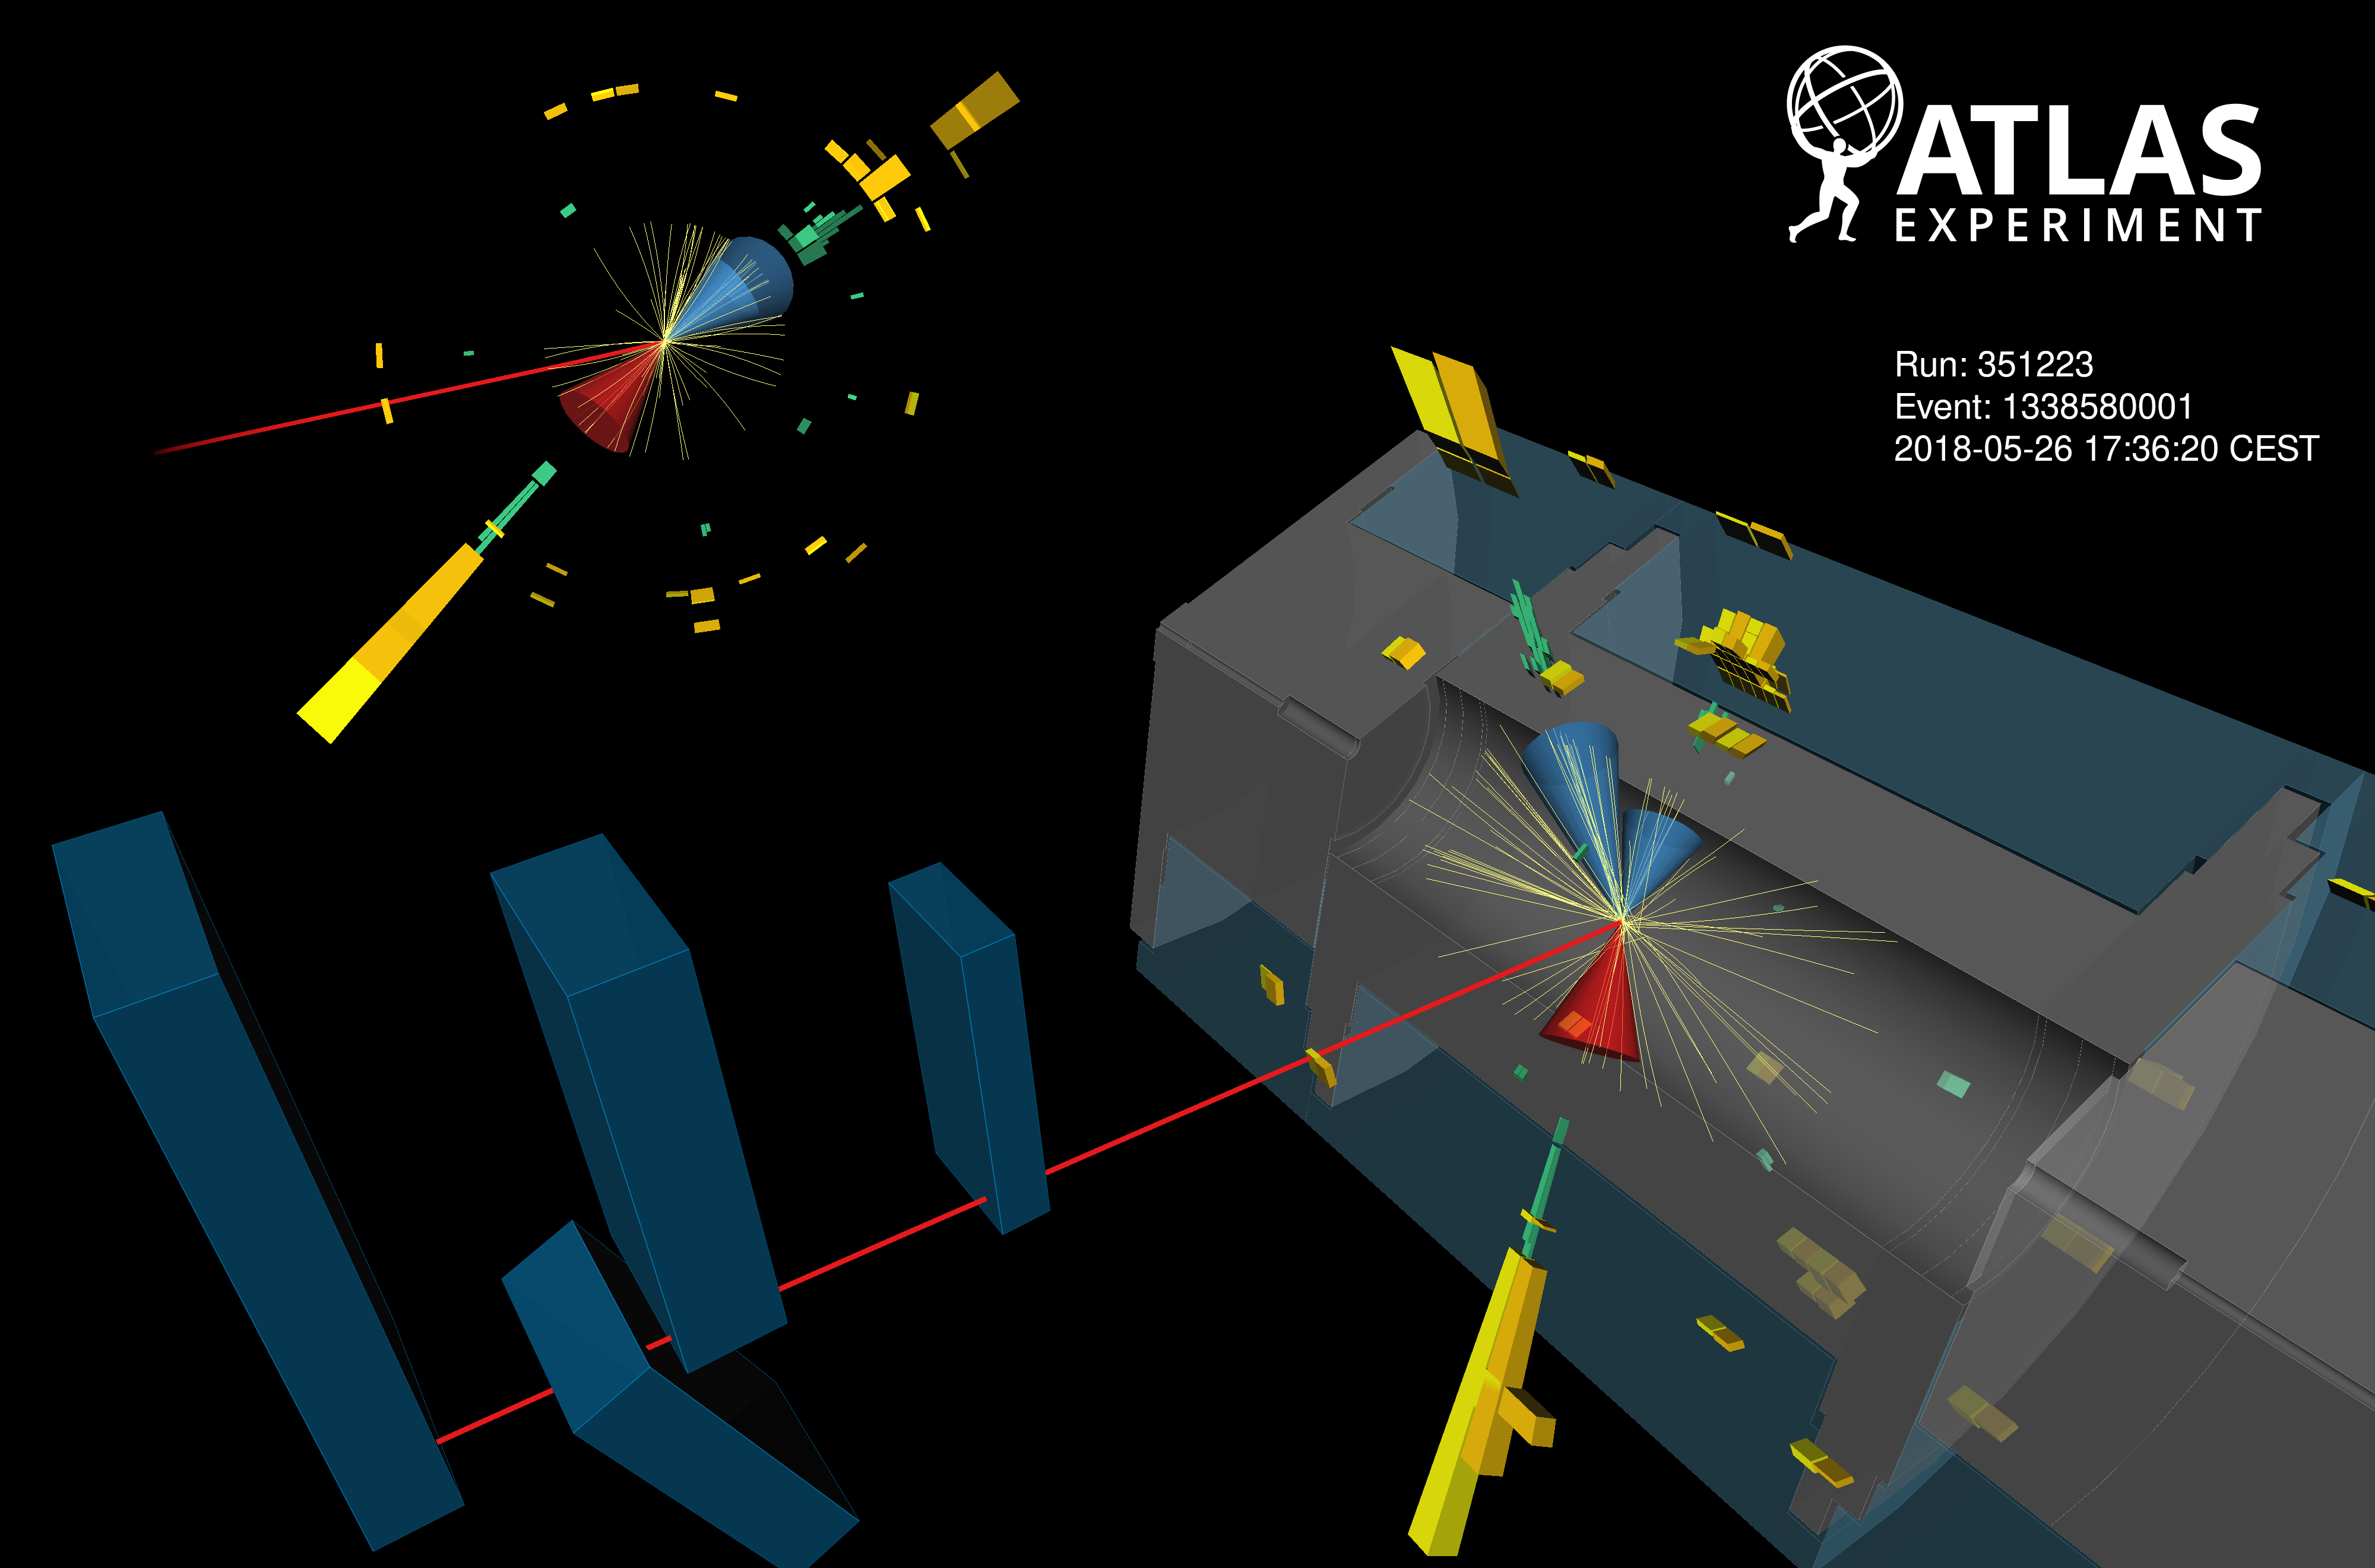
\includegraphics[keepaspectratio,
        width=\paperwidth,
        height=\paperheight]{event_displays/lephad}
      };
      % \node at (0.73\paperwidth,0.46\paperheight) {
      %   \textcolor{White}{$HH \ra {\color{bjetblue}b\bar{b}}{\color{taured}\tauhad\tauhad}$ candidate event}
      % };
    \end{tikzpicture}
  \end{frame}
}

% ------------------------------------------------------------------------------

\begin{frame}[standout]
  Backup
\end{frame}

% ------------------------------------------------------------------------------

\begin{frame}{Pre-Fit Yield Table}
  \centering

  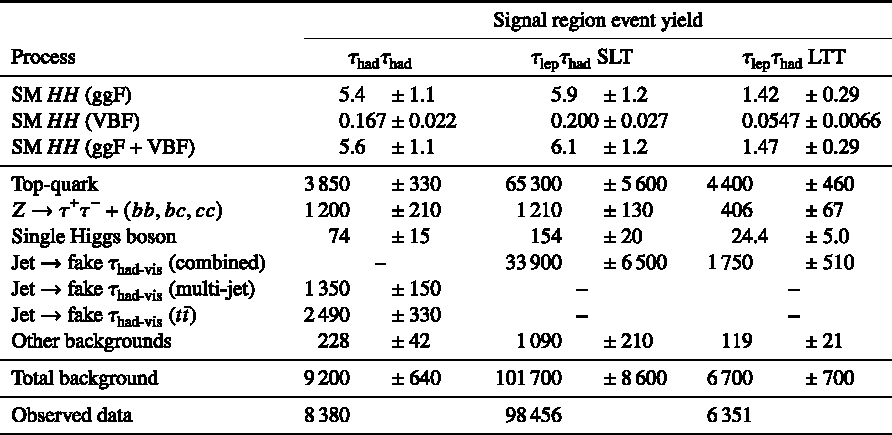
\includegraphics[width=0.9\textwidth]{yieldtable_prefit}
\end{frame}

\begin{frame}{Post-Fit Yield Table}
  \centering

  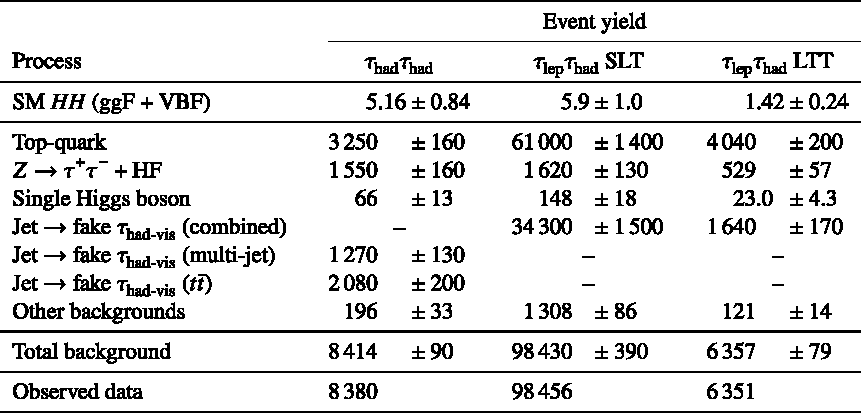
\includegraphics[width=0.9\textwidth]{yieldtable_postfit}
\end{frame}

\end{document}

%%% Local Variables:
%%% mode: latex
%%% TeX-master: "talk.tex"
%%% End:
